\section{Multivariable analysis}

\subsection{Samples}
Signal samples:
\begin{itemize}
\item mc15\_13TeV.392415.MGPy8EG\_A14N23LO\_C1N2\_Slep\_400\_300\_0p95\_2L5.merge.DAOD\_SUSY2.e4287\_a766\_a810\_r6282\_p2499\_p2500\_pUM999999
\end{itemize}

Background samples:

Charge flip and fake lepton background are data driven. The GRL $data16_13TeV.periodAllYear\_DetStatus-v823-pro20-15\_DQDefects-00-02-04\_PHYS\_StandardGRL\_All\_Good_25ns.xml$ was used. The 33.26fb-1 data used covers run 297730 to 311481

%FIXME,  should not have a separate section for BDT evt selection, bkg and trig
Wgamma, diboson and ttbar background are from following MC samples:\\
\begin{itemize}
\item 410066	MadGraphPythia8EvtGen\_A14NNPDF23LO\_ttW\_Np0
\item 410067	MadGraphPythia8EvtGen\_A14NNPDF23LO\_ttW\_Np1
\item 410068	MadGraphPythia8EvtGen\_A14NNPDF23LO\_ttW\_Np2
\item 410112	MadGraphPythia8EvtGen\_A14NNPDF23LO\_ttee\_Np1
\item 410115	MadGraphPythia8EvtGen\_A14NNPDF23LO\_tttautau\_Np0
\item 410114	MadGraphPythia8EvtGen\_A14NNPDF23LO\_ttmumu\_Np1
\item 410113	MadGraphPythia8EvtGen\_A14NNPDF23LO\_ttmumu\_Np0
\item 410111	MadGraphPythia8EvtGen\_A14NNPDF23LO\_ttee\_Np0
\item 410116	MadGraphPythia8EvtGen\_A14NNPDF23LO\_tttautau\_Np1
\item 361063	Sherpa\_CT10\_llll
\item 361064	Sherpa\_CT10\_lllvSFMinus
\item 361065	Sherpa\_CT10\_lllvOFMinus
\item 361066	Sherpa\_CT10\_lllvSFPlus
\item 361067	Sherpa\_CT10\_lllvOFPlus
\item 361068	Sherpa\_CT10\_llvv
\item 361069	Sherpa\_CT10\_llvvjj\_ss\_EW4
\item 361070	Sherpa\_CT10\_llvvjj\_ss\_EW6
\item 361071	Sherpa\_CT10\_lllvjj\_EW6
\item 361072	Sherpa\_CT10\_lllljj\_EW6
\item 301890	Sherpa\_CT10\_enugammaPt35\_70
\item 301891	Sherpa\_CT10\_enugammaPt70\_140
\item 301892	Sherpa\_CT10\_enugammaPt140
\item 301893	Sherpa\_CT10\_munugammaPt35\_70
\item 301894	Sherpa\_CT10\_munugammaPt70\_140
\item 301895	Sherpa\_CT10\_munugammaPt140
\item 301896	Sherpa\_CT10\_taunugammaPt35\_70
\item 301897	Sherpa\_CT10\_taunugammaPt70\_140
\item 301898	Sherpa\_CT10\_taunugammaPt140
\end{itemize}

Data Selection:\\
The follow filters are applied to the data 
\begin{description}


\item [nPrimaryVertex>0] a Vertex need 2+ tracks with pT 2+GeV to be accepted as a primaryVertex
\item [GRL]
\item [“Standard” object definition] \ \\
Tight e TightLLH, Et<20GeV, eta<2.47 \\
Tight mu Medium, pT<25GeV, eta<2.7 \\
and others\\

\item [Exactly 2 lepton]
\item [triggerCut] \ \\

muonTrig =["HLT\_mu26\_imedium", "HLT\_mu24\_imedium", "HLT\_mu24\_iloose\_L1MU15","HLT\_mu20\_iloose\_L1MU15", "HLT\_mu50", "HLT\_mu60\_0eta105\_msonly"]\\

dimuonTrig = ["HLT\_2mu14","HLT\_2mu10","HLT\_mu24\_mu8noL1","HLT\_mu22\_mu8noL1","HLT\_mu20\_mu8noL1","HLT\_mu18\_mu8noL1"]\\

trimuonTrig = ["HLT\_mu24\_2mu4noL1","HLT\_mu22\_2mu4noL1","HLT\_mu20\_2mu4noL1","HLT\_mu18\_2mu4noL1","HLT\_3mu6","HLT\_3mu6\_msonly"]\\

electronTrigCut = ["HLT\_e26\_tight\_iloose","HLT\_e60\_medium","HLT\_e24\_tight\_iloose","HLT\_e24\_medium\_iloose\_L1EM20VH","HLT\_e24\_medium\_iloose\_L1EM18VH"]\\

electronTrigLH = ["HLT\_e26\_lhtight\_iloose","HLT\_e60\_lhmedium","HLT\_e24\_lhtight\_iloose","HLT\_e24\_lhmedium\_iloose\_L1EM20VH","HLT\_e24\_lhmedium\_iloose\_L1EM18VH"]\\

dielectronTrigCut = ["HLT\_2e17\_loose","HLT\_2e15\_loose\_L12EM13VH","HLT\_2e12\_loose\_L12EM10VH"]\\

dielectronTrigLH = ["HLT\_2e17\_lhloose","HLT\_2e15\_lhloose\_L12EM13VH","HLT\_2e12\_lhloose\_L12EM10VH"]\\

trielectronTrigCut = ["HLT\_e17\_medium\_2e9\_medium"]\\

trielectronTrigLH = ["HLT\_e17\_lhmedium\_2e9\_lhmedium"]\\

elemuonTrigCut = ["HLT\_e17\_loose\_mu14","HLT\_e7\_medium\_mu24","HLT\_e26\_medium\_L1EM22VHI\_mu8noL1","HLT\_e24\_medium\_L1EM20VHI\_mu8noL1"]\\

elemuonTrigLH = ["HLT\_e17\_lhloose\_mu14","HLT\_e7\_lhmedium\_mu24","HLT\_e26\_lhmedium\_L1EM22VHI\_mu8noL1","HLT\_e24\_lhmedium\_L1EM20VHI\_mu8noL1"]\\

trielemuonTrigCut = ["HLT\_e12\_loose\_2mu10","HLT\_2e12\_loose\_mu10"]\\

trielemuonTrigLH = ["HLT\_e12\_lhloose\_2mu10","HLT\_2e12\_lhloose\_mu10"]\\

\item [0 Bjet]\ \\
\item [0 cosmic mu]\ \\
\end{description}


\subsection{Variables}
BDT Training:\\
We separate out two event types, the ISR region is defined as events having >=1 jets, and the nonISR region which are events with no jets.

The signals are grouped with the Slep mass splitting to 4 types; dm20, dm50 , dm100 and dm100up.

With 2 event types and 4 signal types, we train 8 Boosted Decision Tree in total to classify signal event from background. The BDTD algo in ROOT's TMVA package was used for the job, where BDTD stands for Boosted Decision Tree with decorrelated variables. 

In the nonISR region the following variables are used as input:
\begin{itemize}
\item mT2
\item $pT_{dilepton}$
\item $E_{T}^{Miss,rel}$
\item $H_T$ (scalar sum for 2l+jets pT)
\item $m_{T,l1}$ (transvers mass with leading lepton)
\item $m_{T,l2}$ (transvers mass with 2nd leading lepton)
\item $dPhi_{(l1,l2)}$
\item l12m(dilepton mass)

\end{itemize}

In the ISR region the following extra variables are also used:
\begin{itemize}
\item $dPhi_{(Etmissrel,leading jet)}$
\item $E_T^{miss,rel}/p_{T,leading jet}$
\item $p_{T,l1}/p_{T,leading jet}$
\end{itemize}

%FIXME, choose one particular BDT (eg ISR dm50) and update the plot
The correlation of the BDT input variables for signal and background samples are show in fig\ref{fig:BDT_input_corr}

\begin{figure}
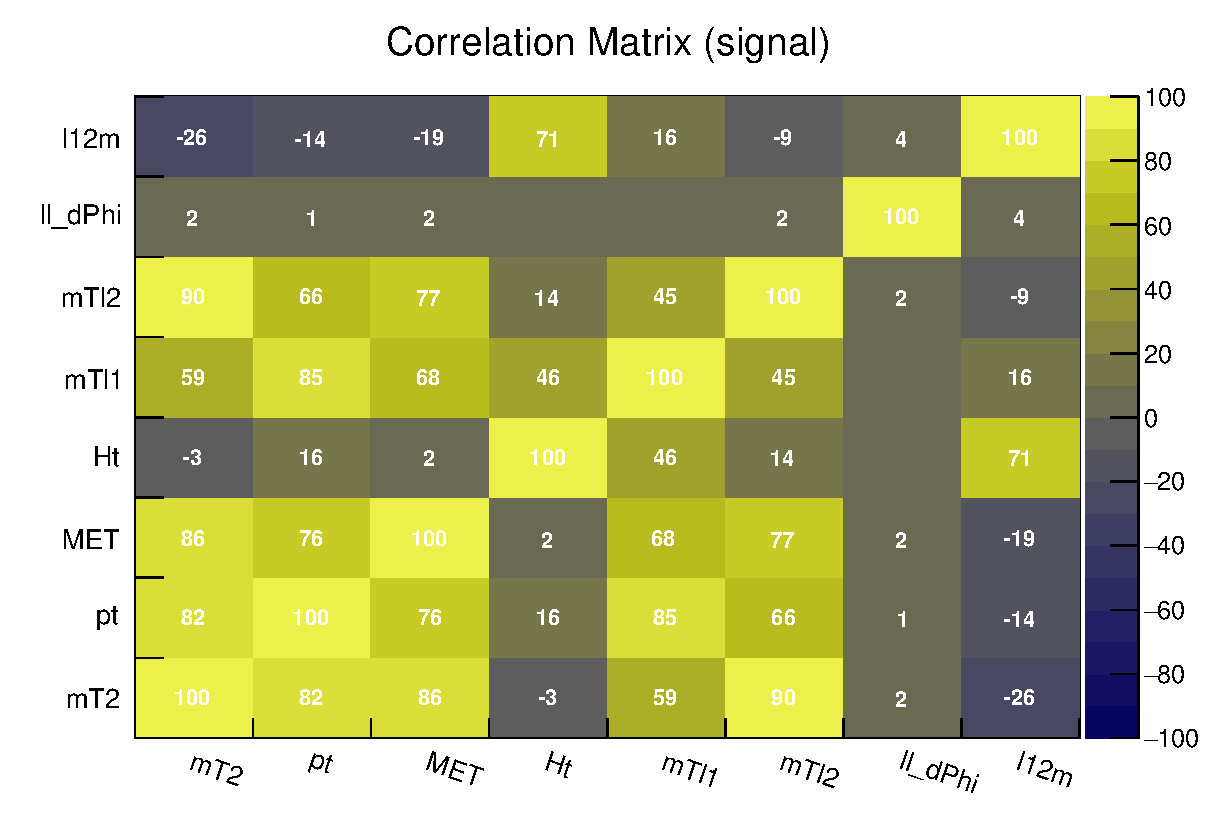
\includegraphics[width=0.5\textwidth]{cutOpt/corrMatS.eps}
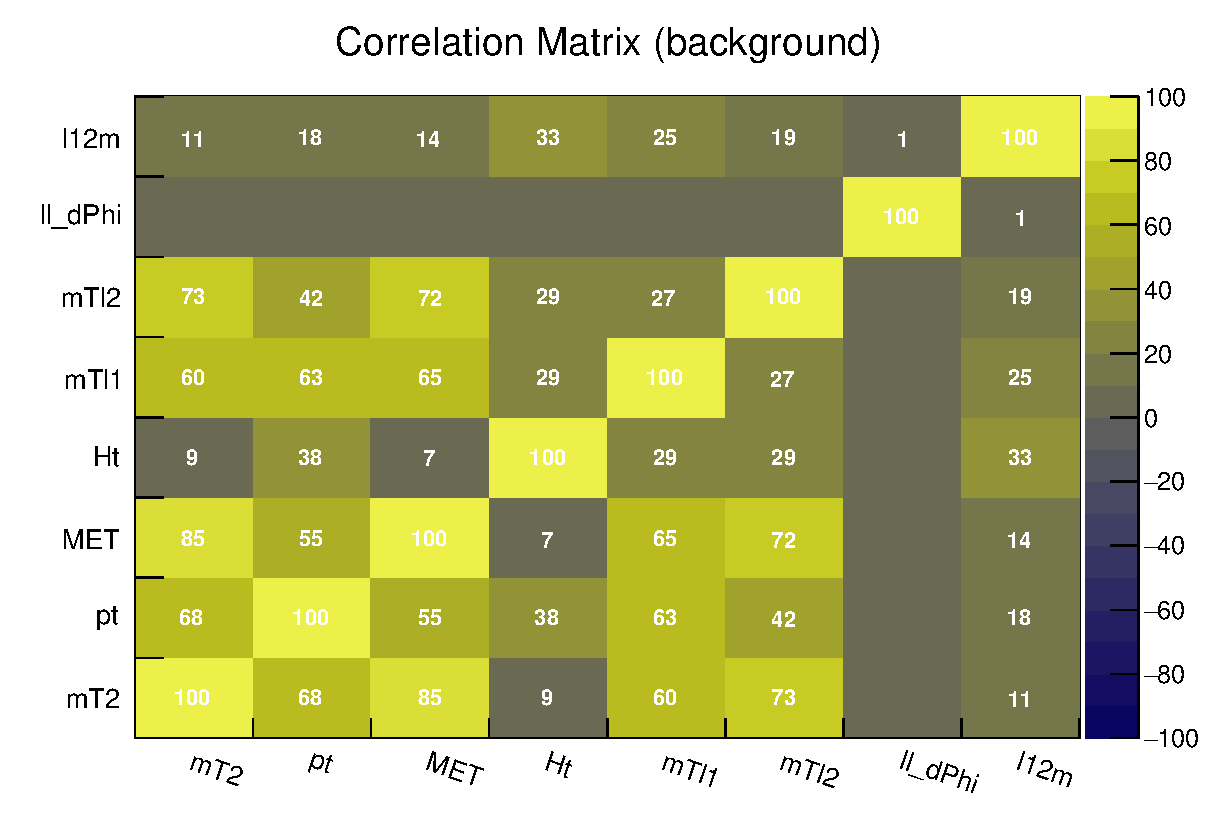
\includegraphics[width=0.5\textwidth]{cutOpt/corrMatB.eps}
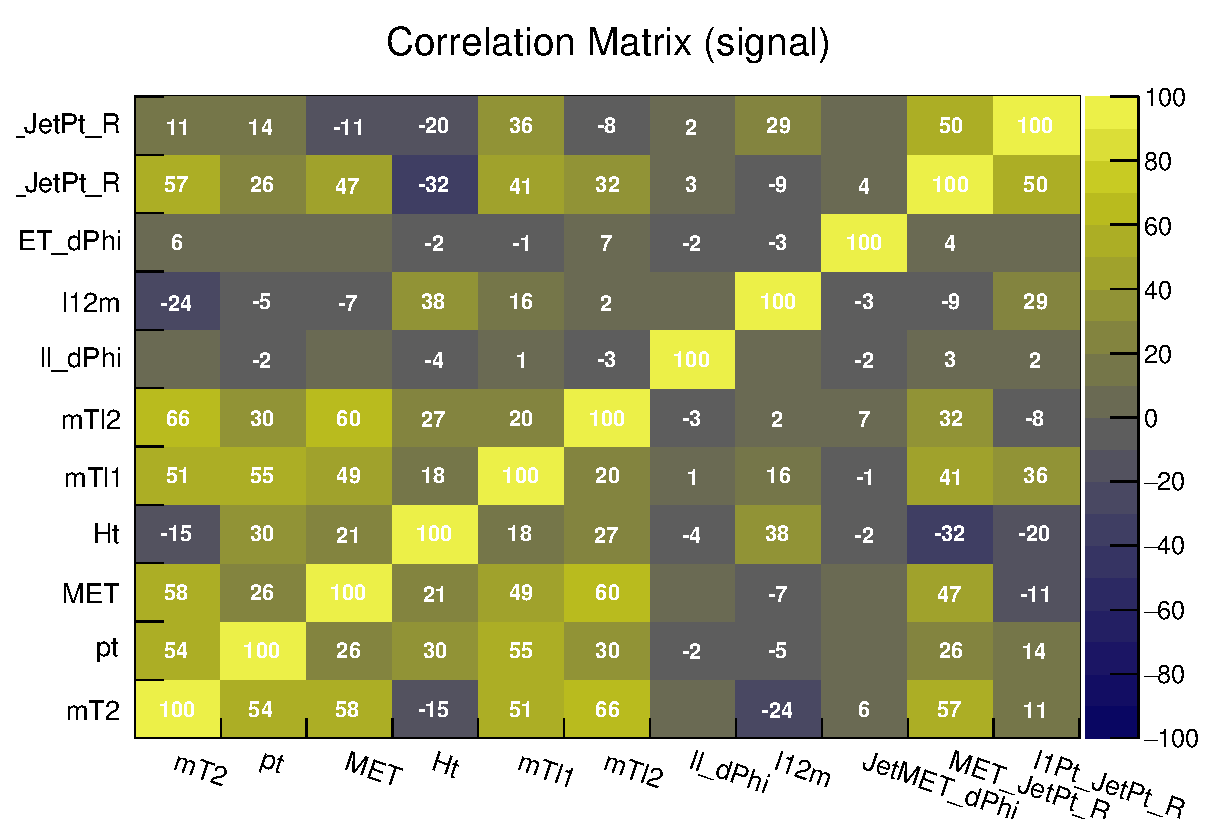
\includegraphics[width=0.5\textwidth]{cutOpt/corrMatS_ISR.eps}
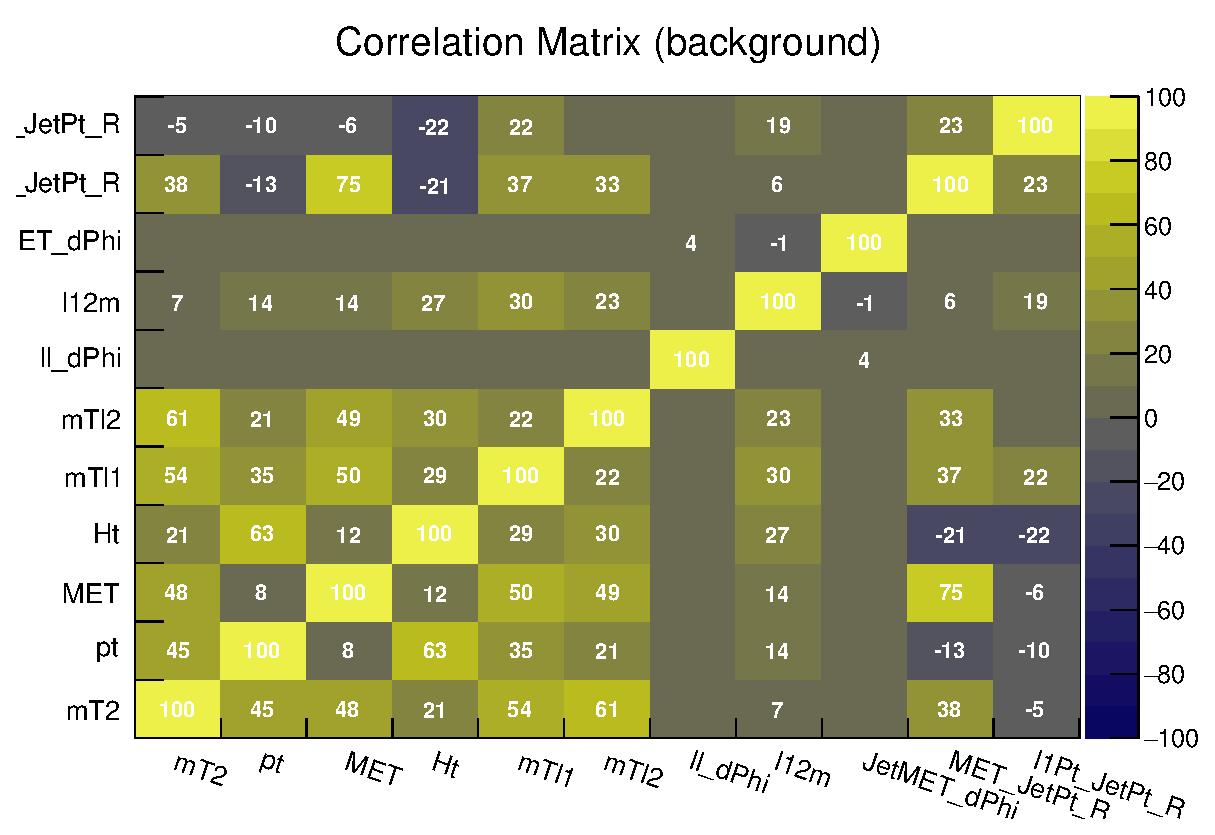
\includegraphics[width=0.5\textwidth]{cutOpt/corrMatB_ISR.eps}
\caption{BDT input variables correlations}
\label{fig:BDT_input_corr}
\end{figure}


The distribution of the BDT input for signal and background samples are show in fig\ref{fig:BDT_nonISR_input}, \ref{fig:BDT_ISR_input}

\begin{figure}
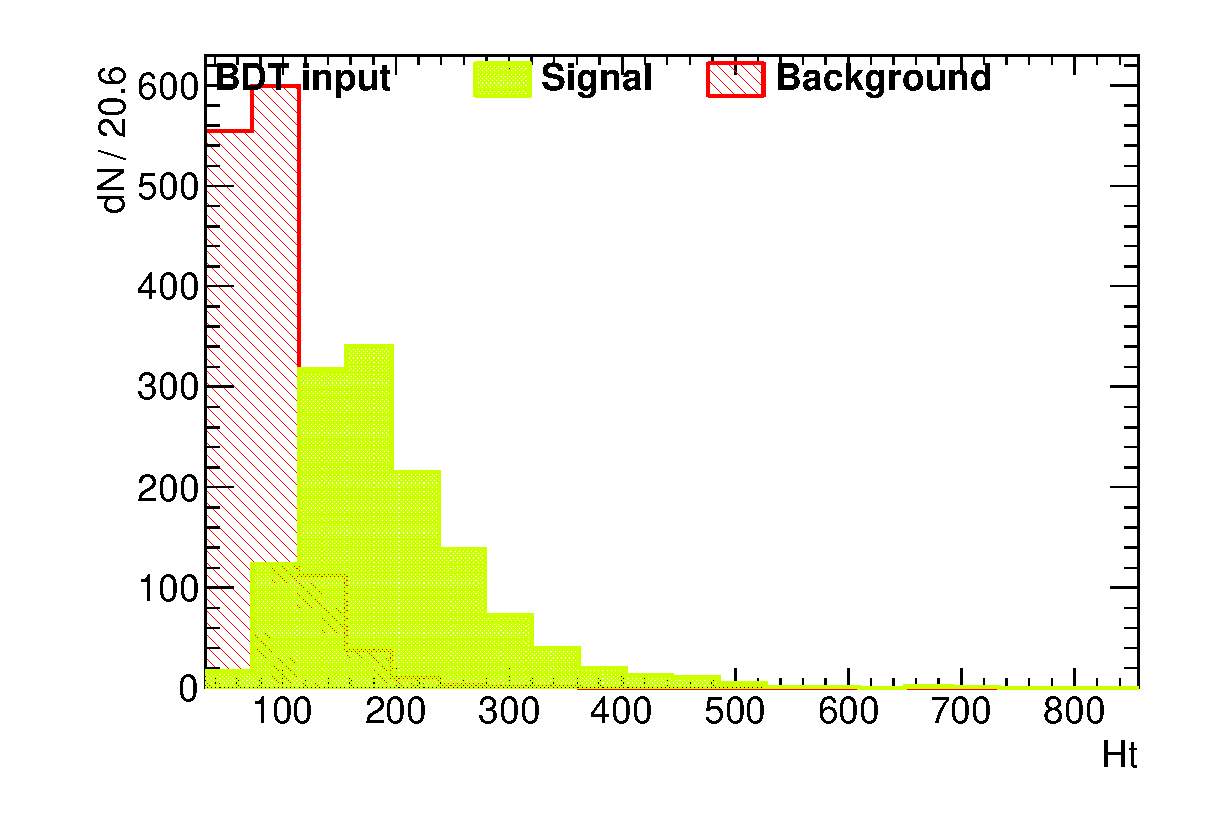
\includegraphics[width=0.5\textwidth]{cutOpt/nonISR_Ht__Signal_Id.eps}
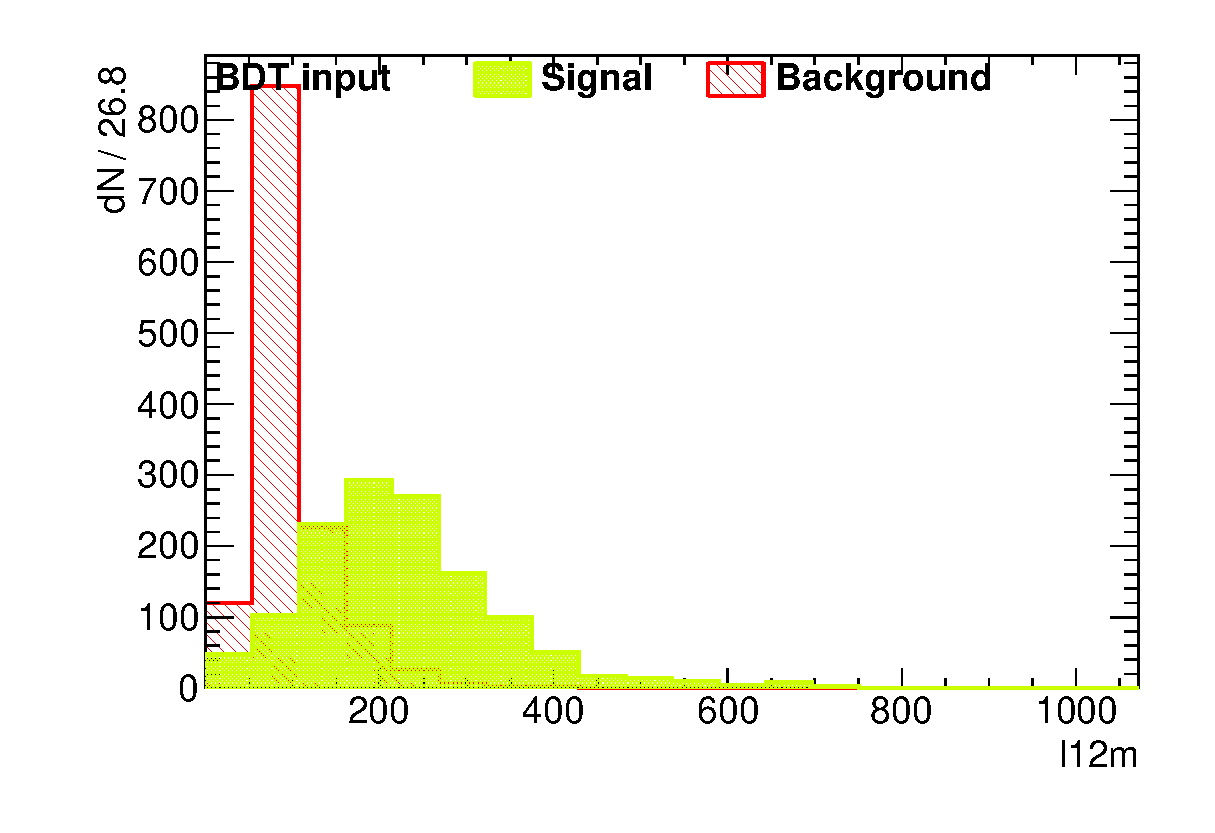
\includegraphics[width=0.5\textwidth]{cutOpt/nonISR_l12m__Signal_Id.eps}
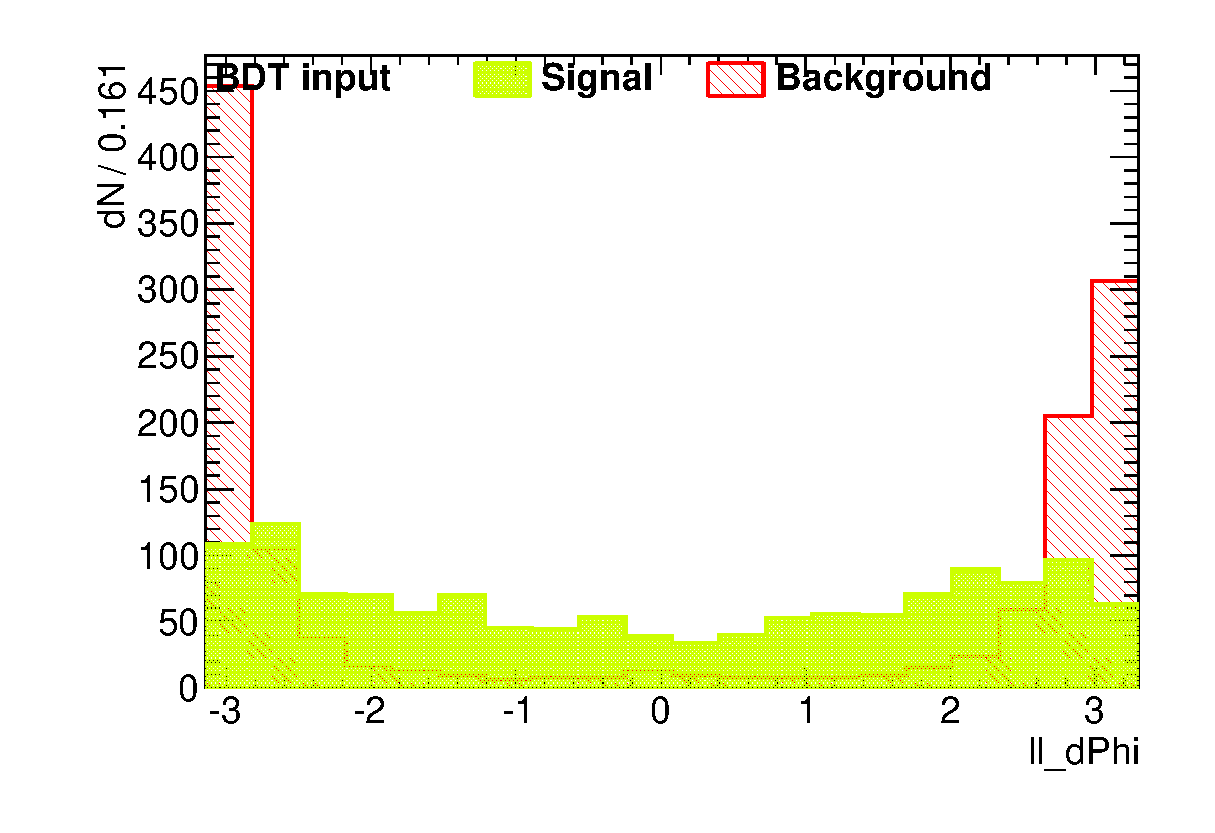
\includegraphics[width=0.5\textwidth]{cutOpt/nonISR_ll_dPhi__Signal_Id.eps}
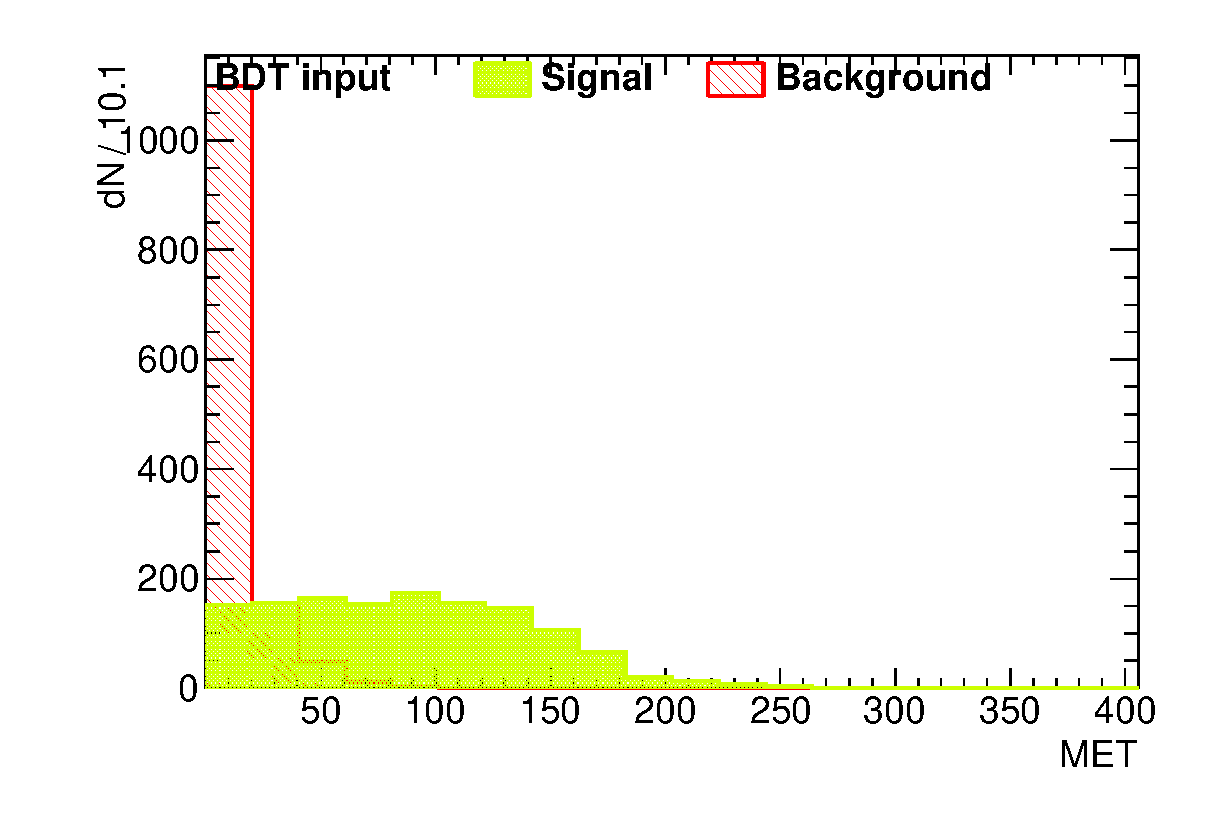
\includegraphics[width=0.5\textwidth]{cutOpt/nonISR_MET__Signal_Id.eps}
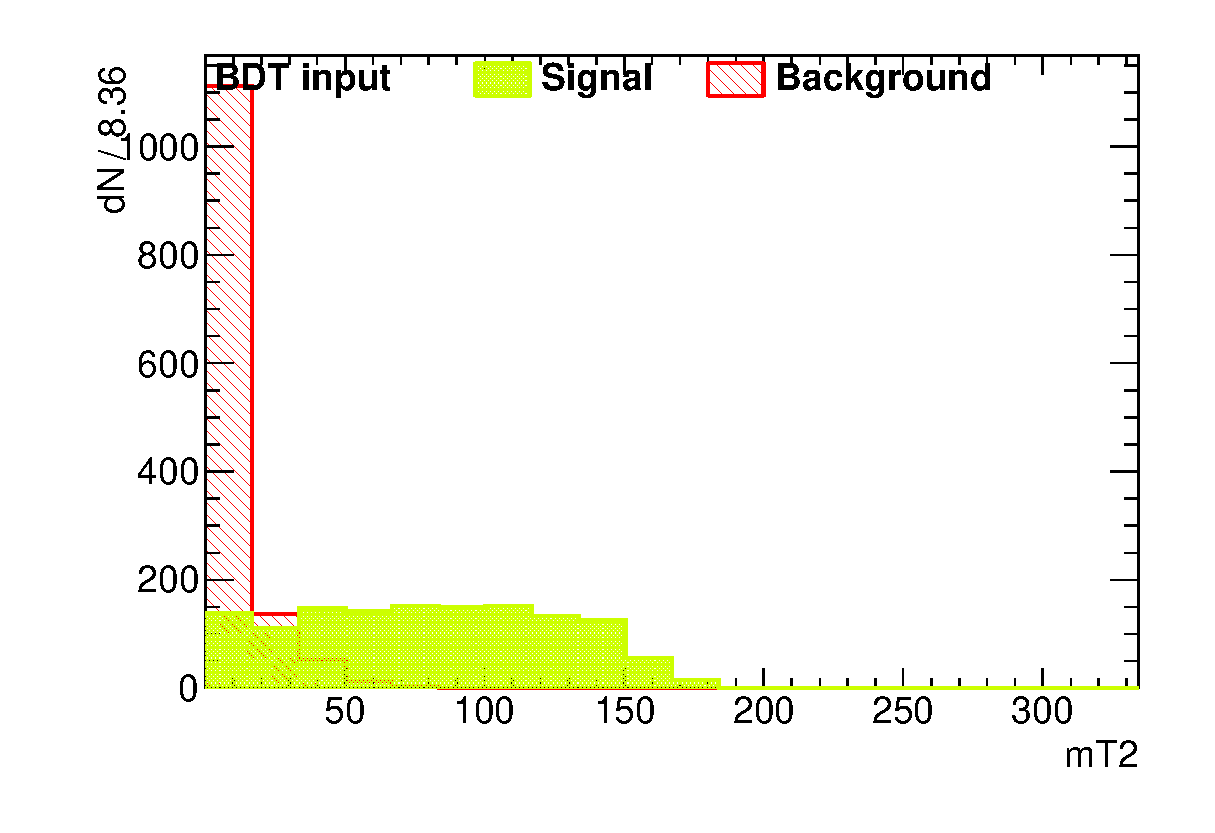
\includegraphics[width=0.5\textwidth]{cutOpt/nonISR_mT2__Signal_Id.eps}
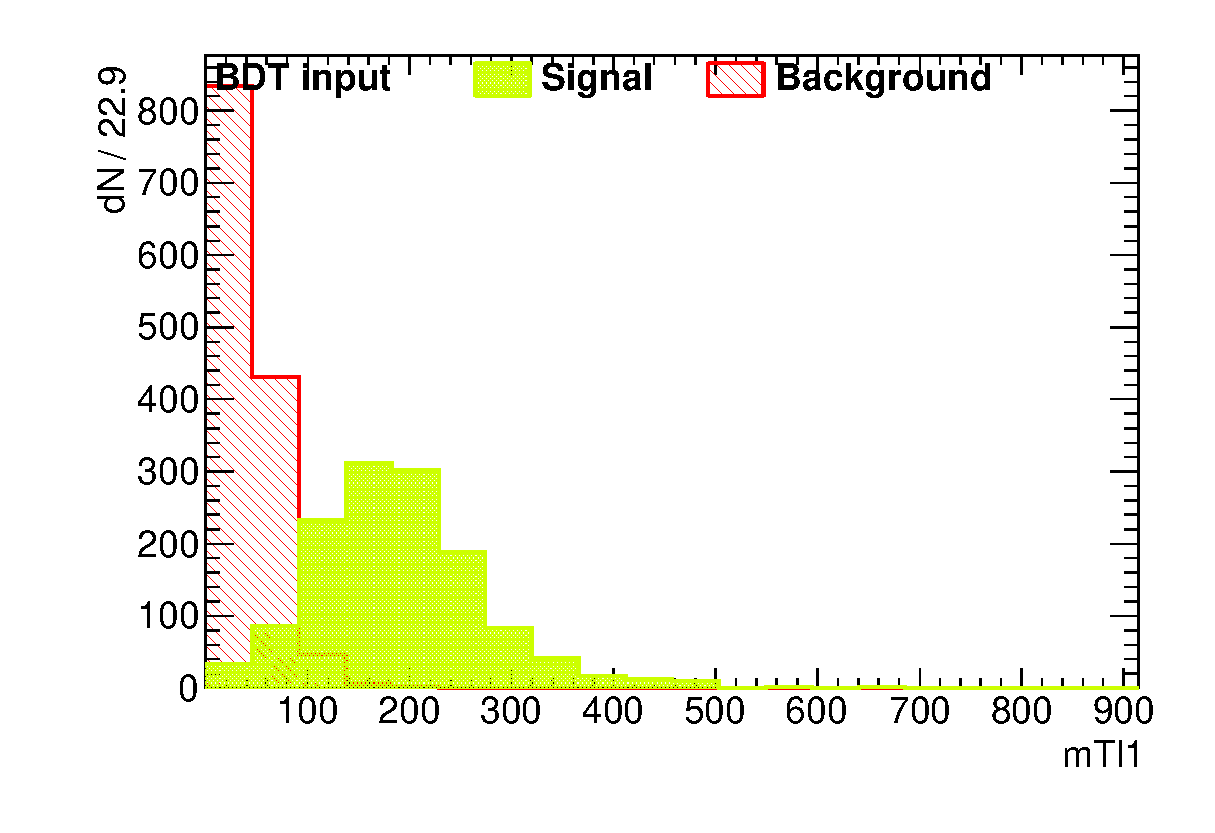
\includegraphics[width=0.5\textwidth]{cutOpt/nonISR_mTl1__Signal_Id.eps}
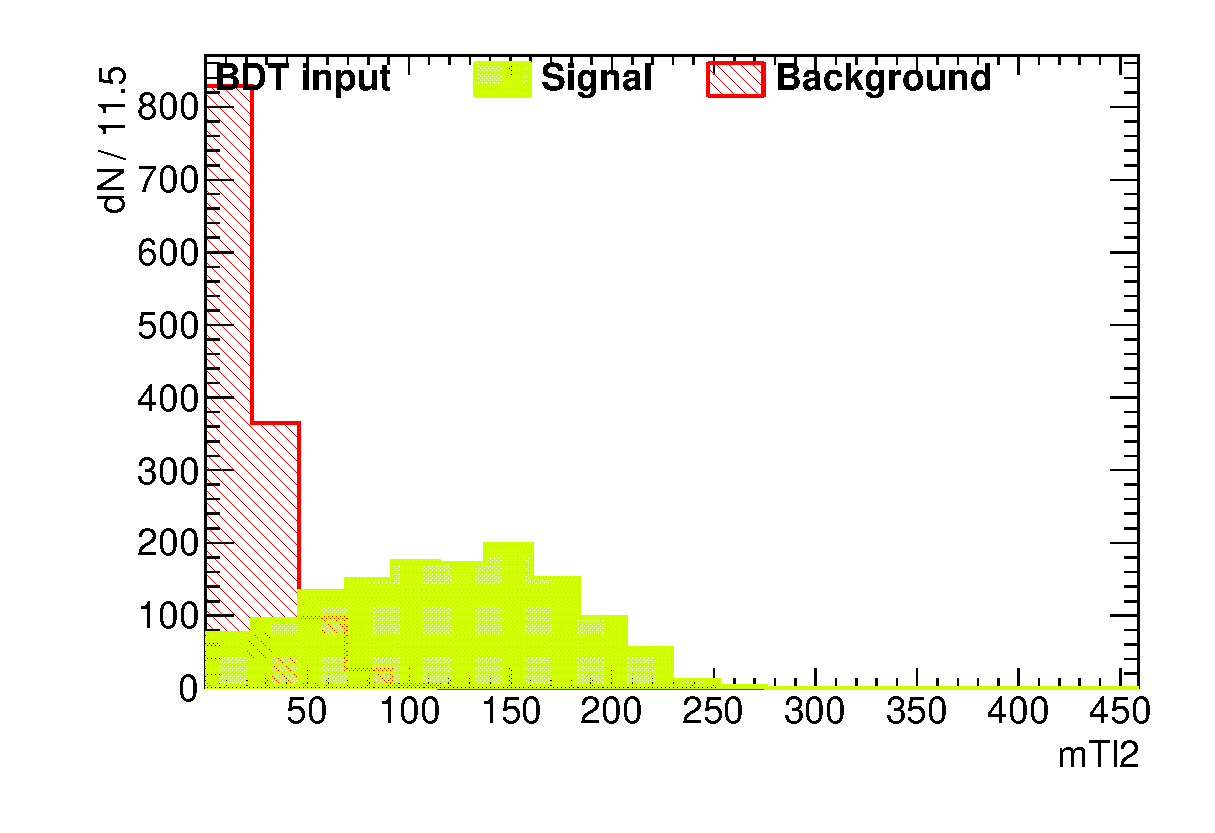
\includegraphics[width=0.5\textwidth]{cutOpt/nonISR_mTl2__Signal_Id.eps}
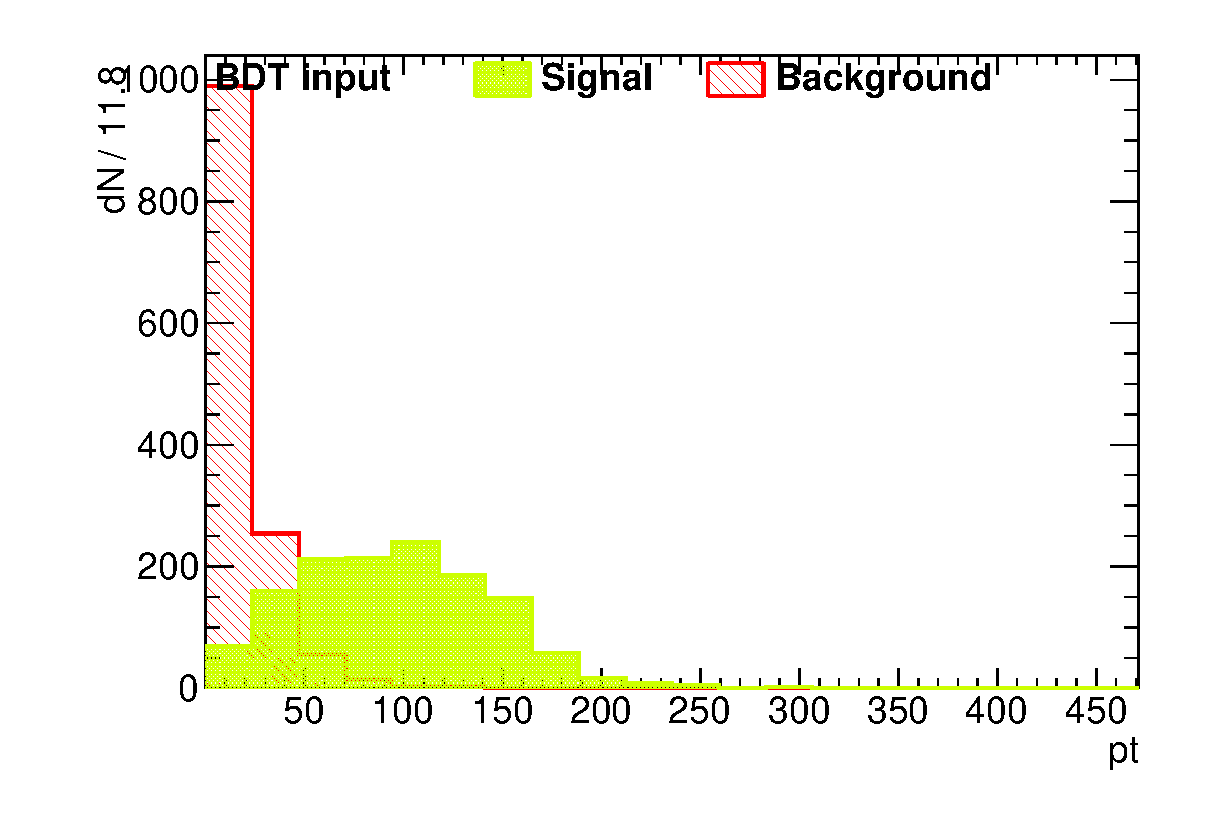
\includegraphics[width=0.5\textwidth]{cutOpt/nonISR_pt__Signal_Id.eps}
\caption{BDT input variables distribution for nonISR region}
\label{fig:BDT_nonISR_input}
\end{figure}

\begin{figure}
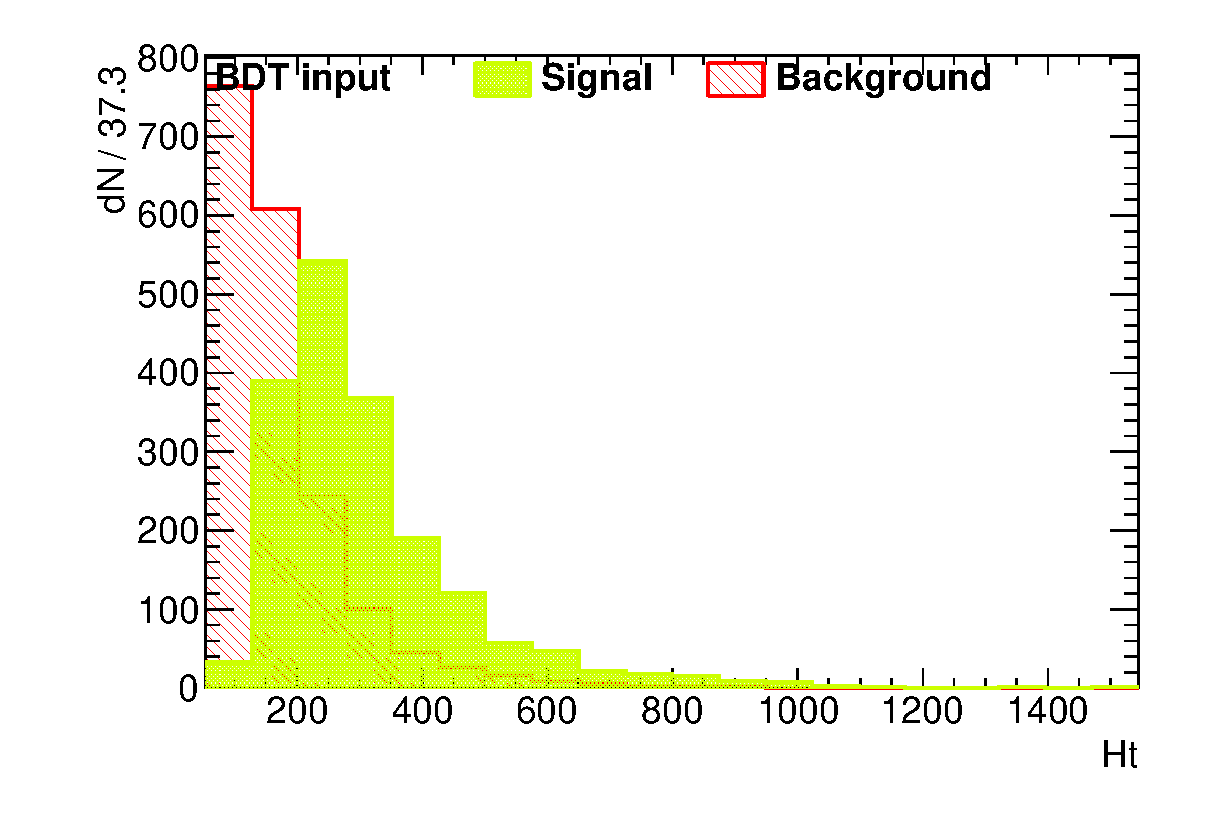
\includegraphics[width=0.5\textwidth]{cutOpt/ISR_Ht__Signal_Id.eps}
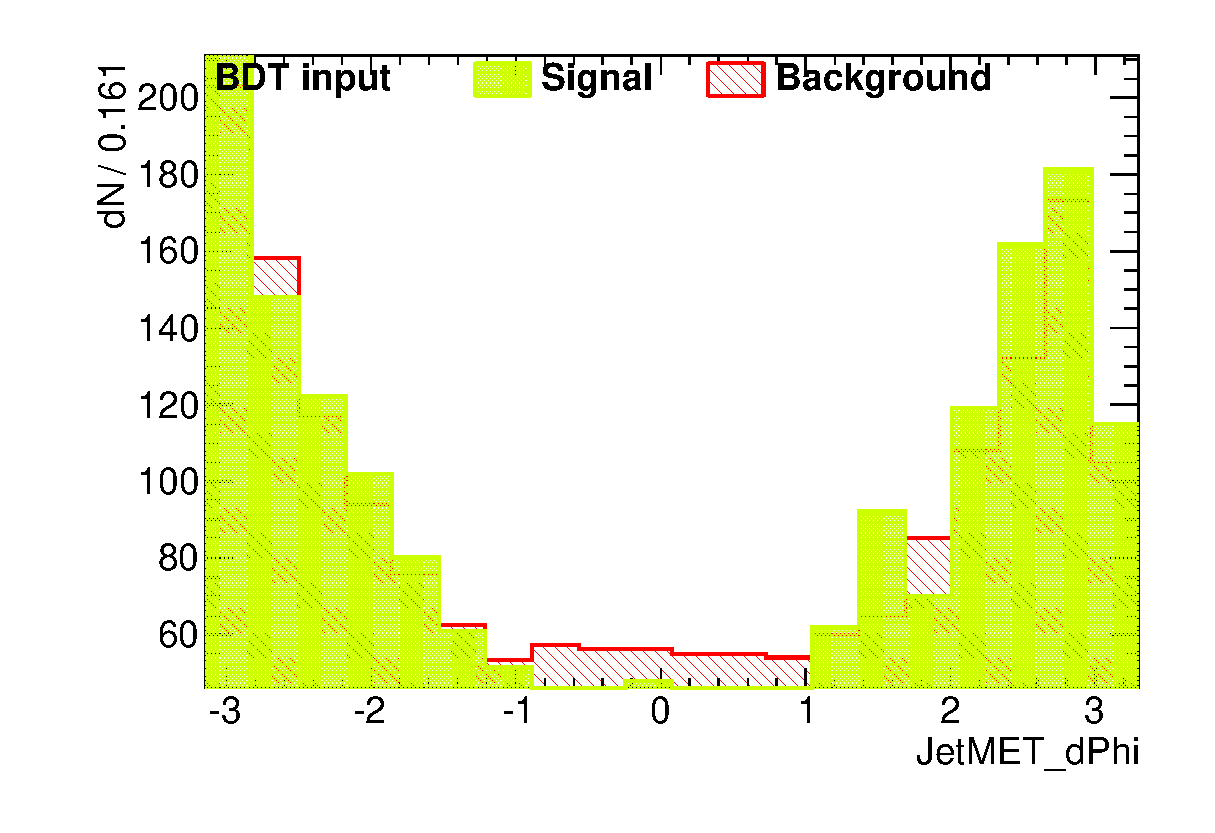
\includegraphics[width=0.5\textwidth]{cutOpt/ISR_JetMET_dPhi__Signal_Id.eps}
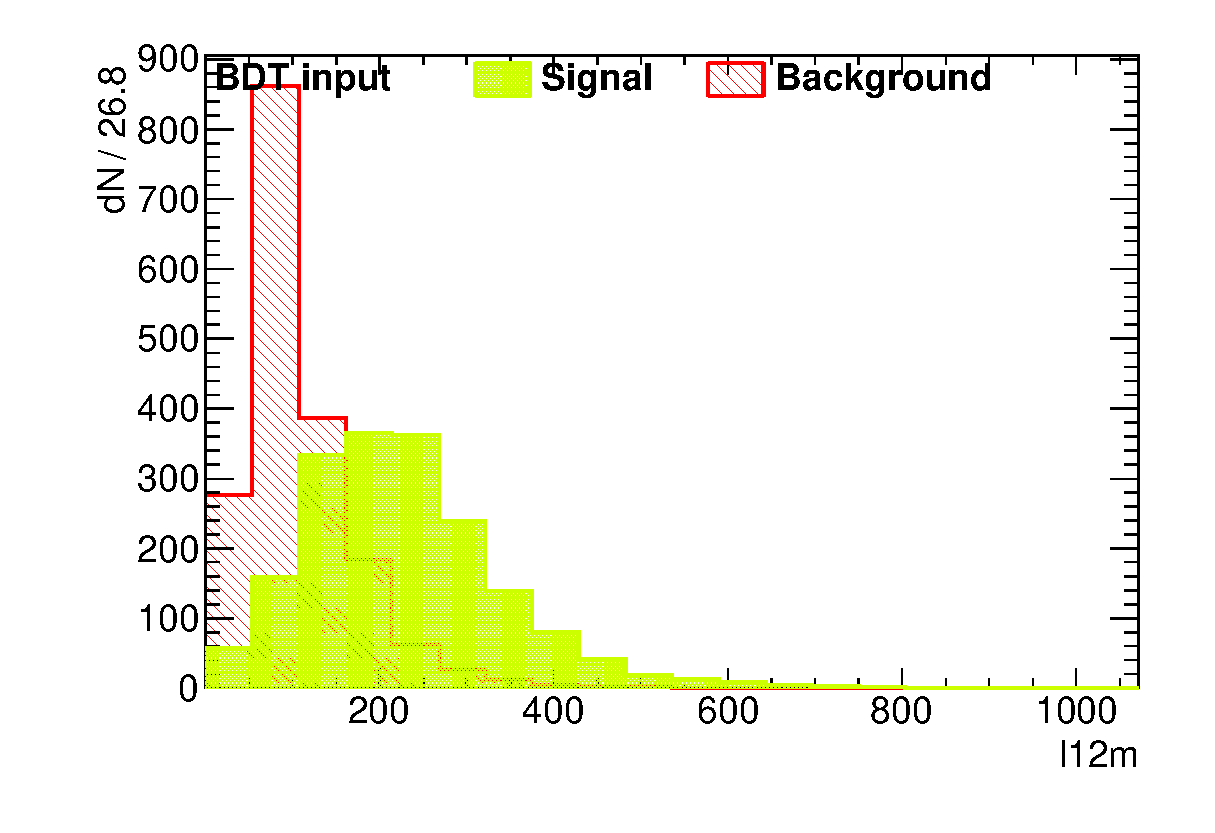
\includegraphics[width=0.5\textwidth]{cutOpt/ISR_l12m__Signal_Id.eps}
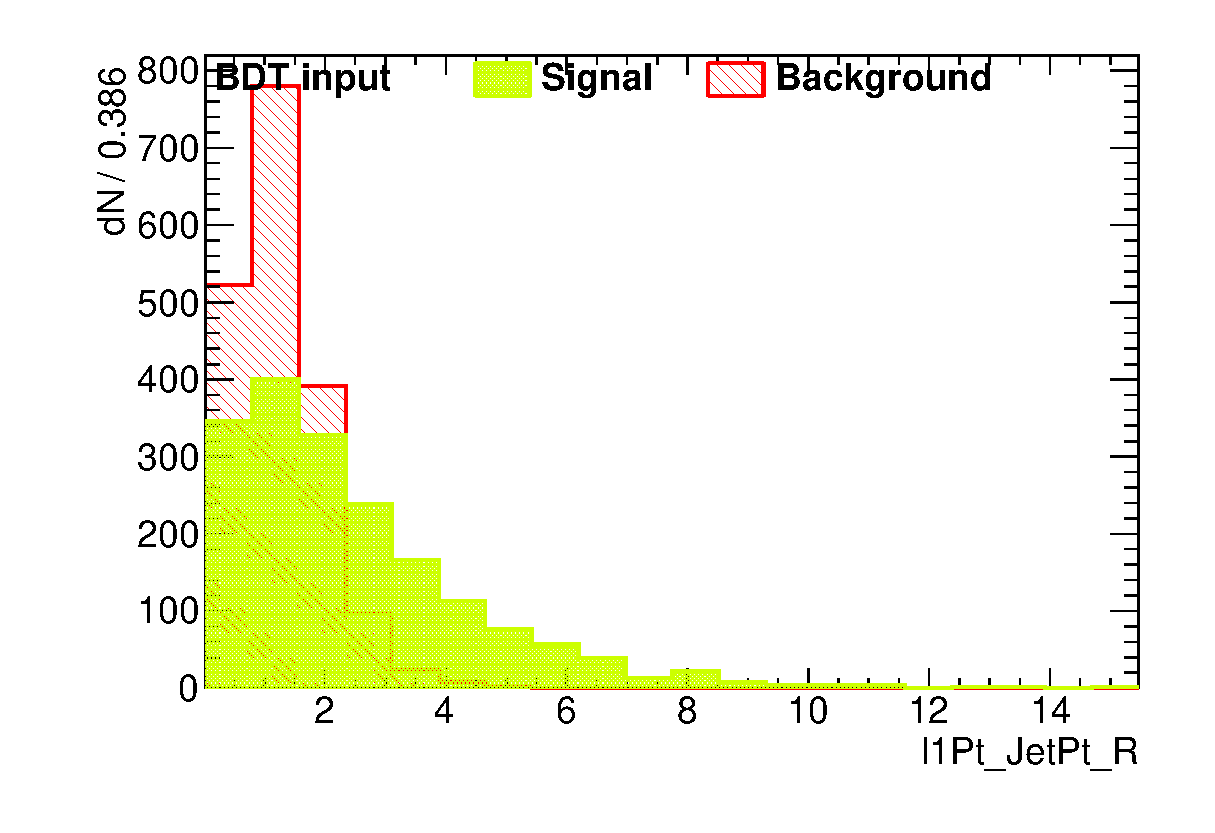
\includegraphics[width=0.5\textwidth]{cutOpt/ISR_l1Pt_JetPt_R__Signal_Id.eps}
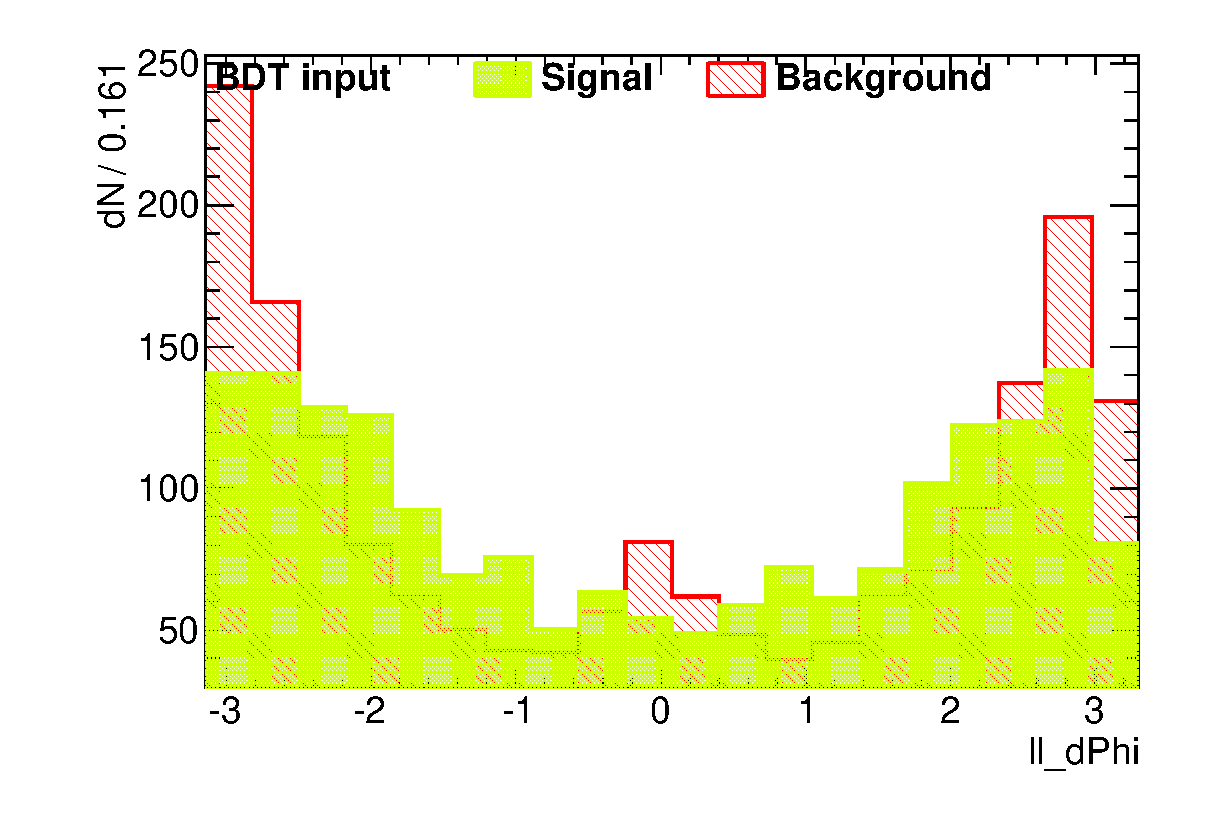
\includegraphics[width=0.5\textwidth]{cutOpt/ISR_ll_dPhi__Signal_Id.eps}
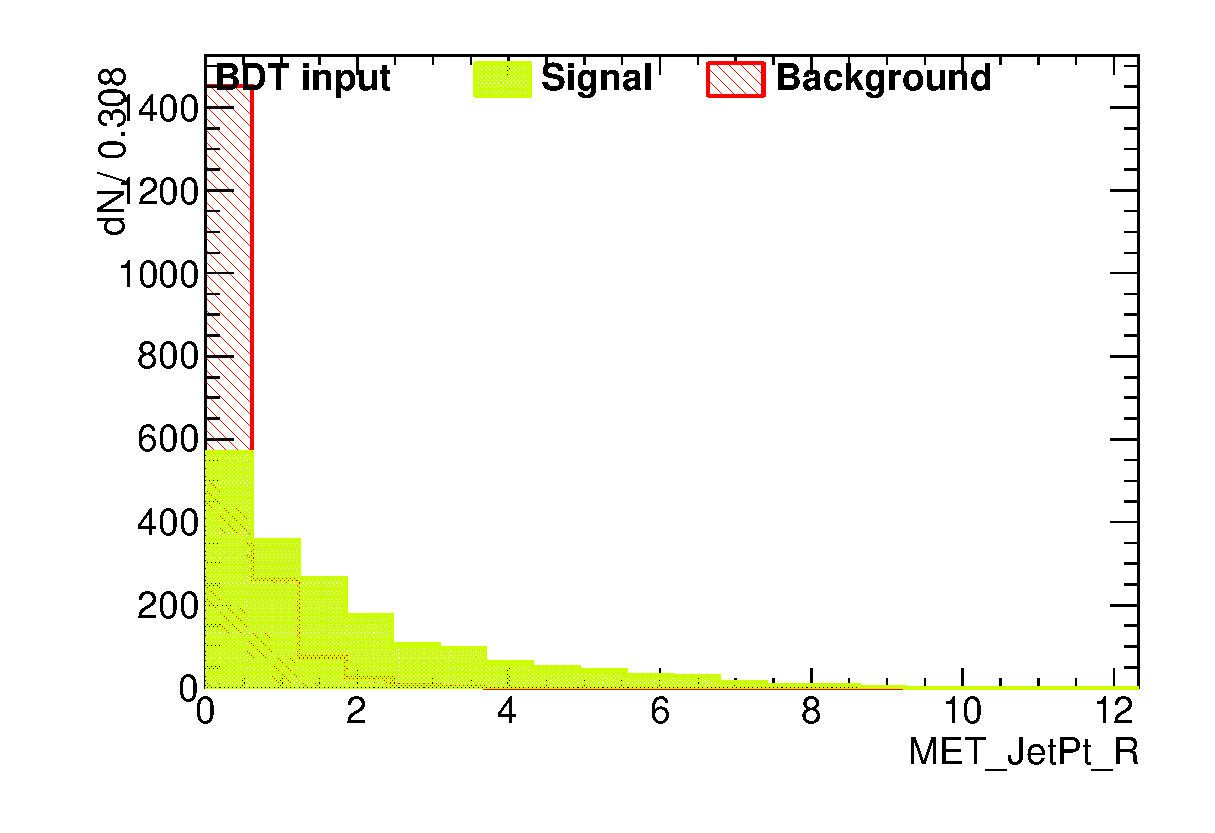
\includegraphics[width=0.5\textwidth]{cutOpt/ISR_MET_JetPt_R__Signal_Id.eps}
\caption{BDT input variables distribution for ISR region}
\label{fig:BDT_ISR_input}
\end{figure}

\begin{figure}
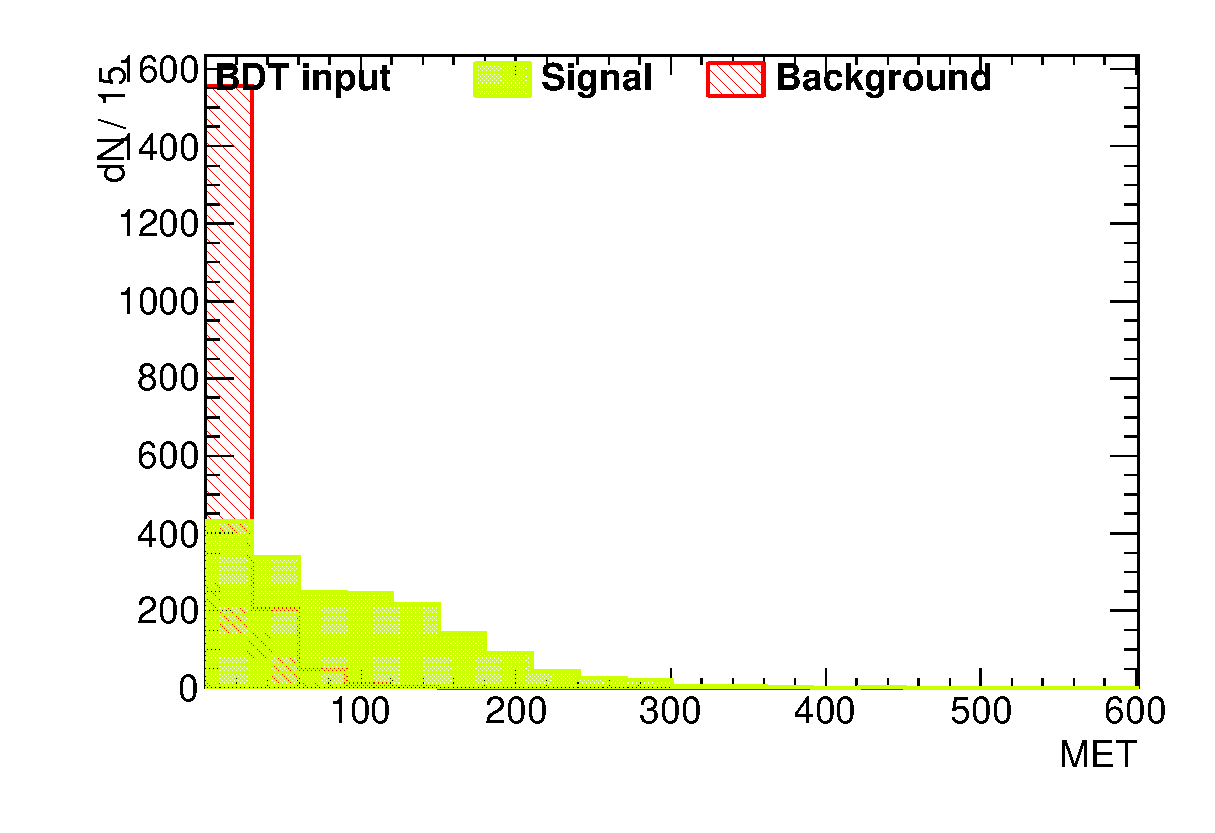
\includegraphics[width=0.5\textwidth]{cutOpt/ISR_MET__Signal_Id.eps}
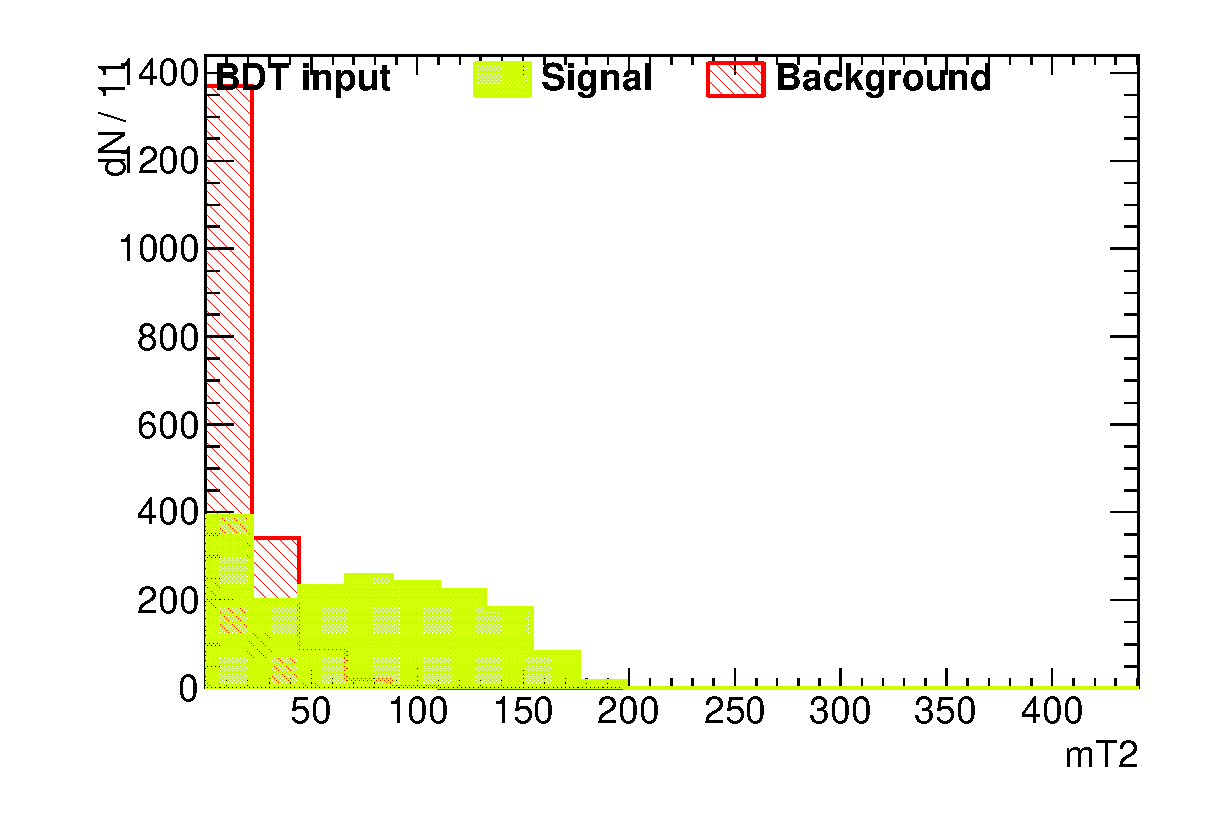
\includegraphics[width=0.5\textwidth]{cutOpt/ISR_mT2__Signal_Id.eps}
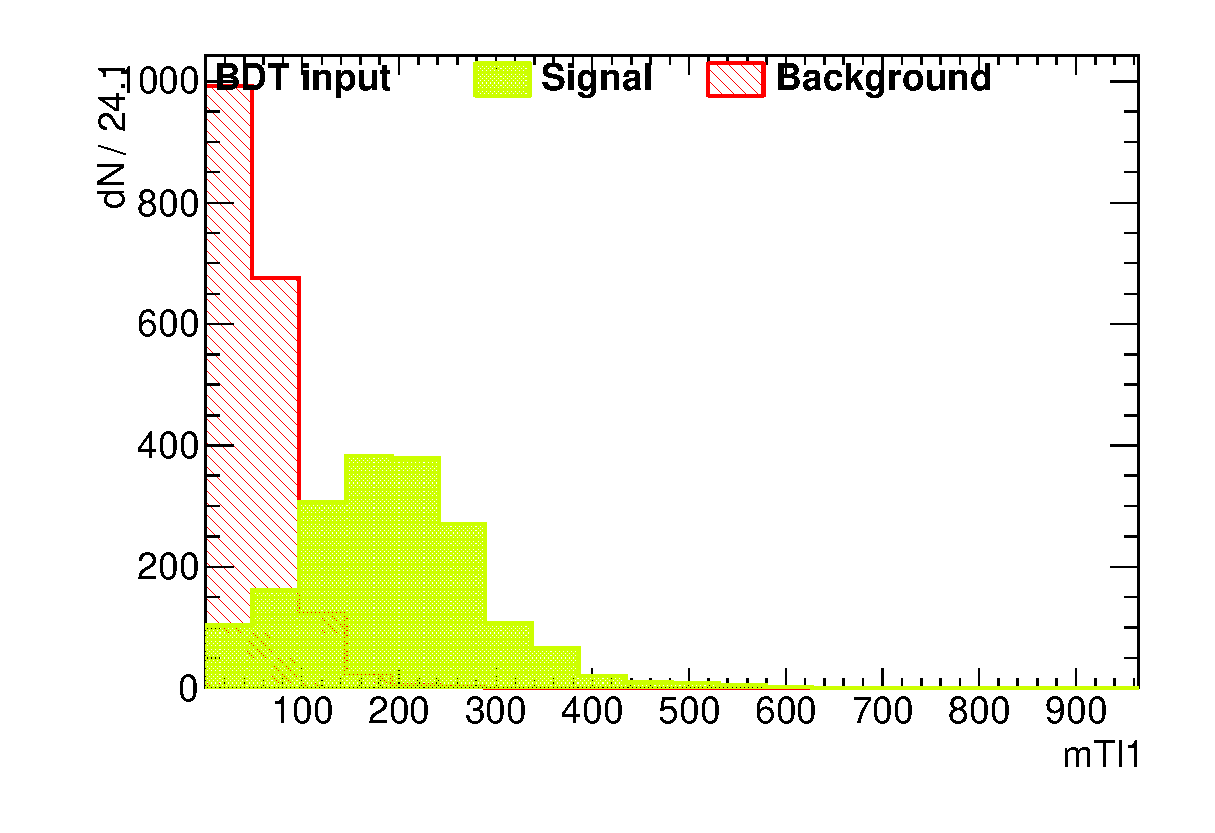
\includegraphics[width=0.5\textwidth]{cutOpt/ISR_mTl1__Signal_Id.eps}
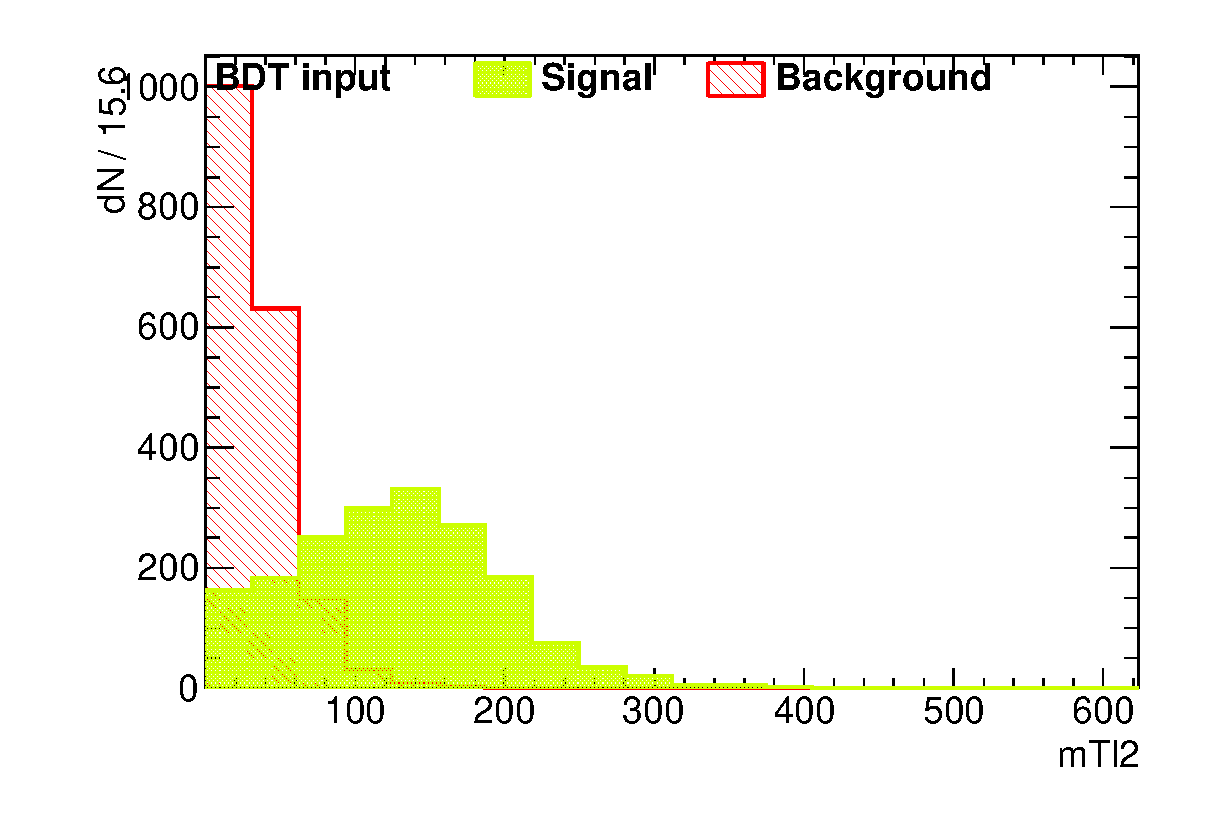
\includegraphics[width=0.5\textwidth]{cutOpt/ISR_mTl2__Signal_Id.eps}
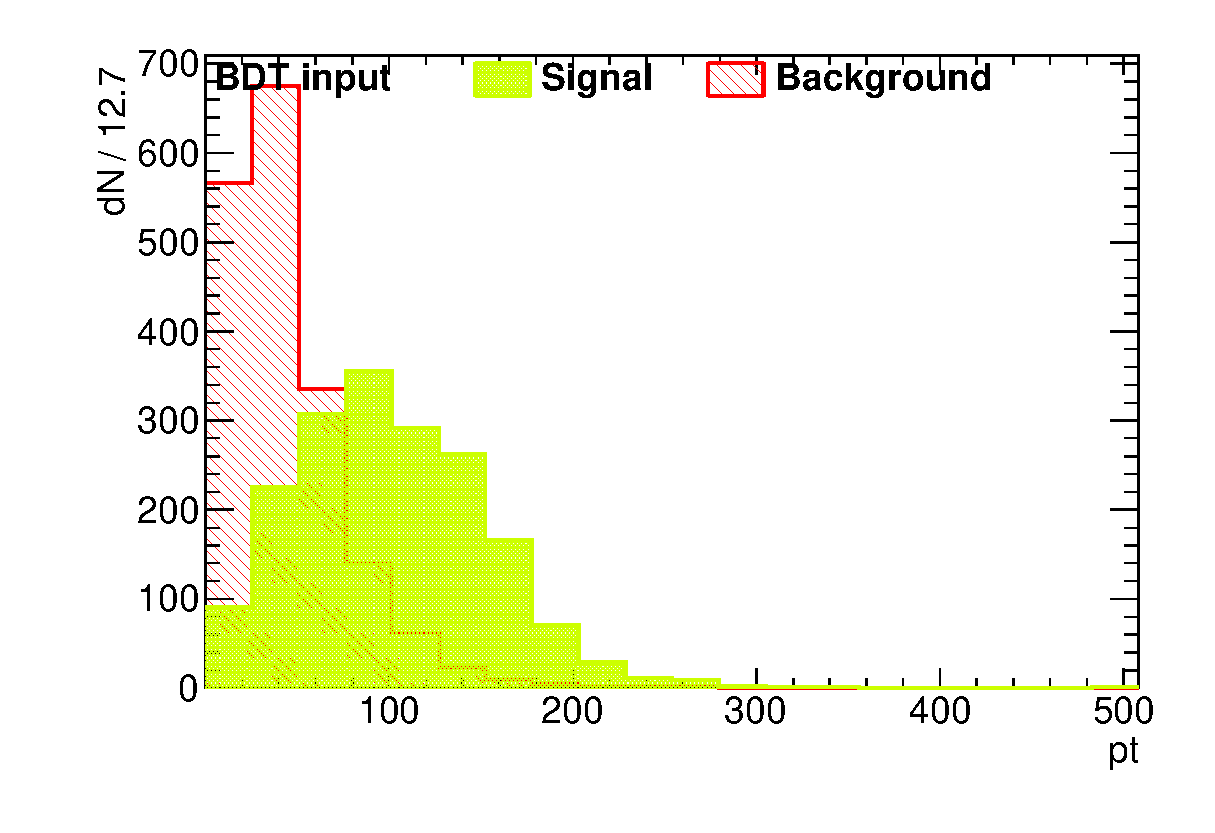
\includegraphics[width=0.5\textwidth]{cutOpt/ISR_pt__Signal_Id.eps}
\caption{BDT input variables distribution for ISR region}
\label{fig:BDT_ISR_input2}
\end{figure}

%FIXME should use Gabriels setting from overtain study
\FloatBarrier
\subsection{BDT parameter selection}
In order to find the best performing BDT parameters, a scan of different BDT parameters were done in various channels for each mass splitting. 

\subsubsection*{Channels}
\begin{itemize}
\item $\Delta m$ = 20, 50, 100 GeV
\item ISR or noISR
\item ee or $\mu\mu$ or e$\mu$ or SF or all flavors
\end{itemize}

\subsubsection*{BDT parameters scanned}
\begin{itemize}
\item NTrees = 100, 200, 400, 600
\item TreeDepth = 2, 3, 4, 5
\item MinNodeSize = 5\%, 7\%, 10\%
\end{itemize}

\subsubsection*{Samples used}
The backgrounds were derived from the MC samples and data-driven methods as specified in a previous part of this appendix. 

The signal samples with the same mass splitting were used to train the respective BDTs in order to maximize the number of available signal samples for training.

\textbf{Signal samples}\\
\tiny
\underline{$\Delta m=20$GeV} \\
\texttt{mc15\_13TeV.392825.MGPy8EG\_A14N23LO\_C1N2\_Slep\_200\_180\_0p95\_2L5.merge.DAOD\_SUSY2.e5129\_a766\_a821\_r7676\_p2688} \\
\texttt{mc15\_13TeV.392826.MGPy8EG\_A14N23LO\_C1N2\_Slep\_300\_280\_0p95\_2L5.merge.DAOD\_SUSY2.e5129\_a766\_a821\_r7676\_p2688} \\
\texttt{mc15\_13TeV.392827.MGPy8EG\_A14N23LO\_C1N2\_Slep\_400\_380\_0p95\_2L5.merge.DAOD\_SUSY2.e5129\_a766\_a821\_r7676\_p2688} \\
\texttt{mc15\_13TeV.392828.MGPy8EG\_A14N23LO\_C1N2\_Slep\_500\_480\_0p95\_2L5.merge.DAOD\_SUSY2.e5129\_a766\_a821\_r7676\_p2688} \\
\texttt{mc15\_13TeV.392829.MGPy8EG\_A14N23LO\_C1N2\_Slep\_600\_580\_0p95\_2L5.merge.DAOD\_SUSY2.e5129\_a766\_a821\_r7676\_p2688} \\
\texttt{mc15\_13TeV.392830.MGPy8EG\_A14N23LO\_C1N2\_Slep\_700\_680\_0p95\_2L5.merge.DAOD\_SUSY2.e5129\_a766\_a821\_r7676\_p2688} \\
\texttt{mc15\_13TeV.392832.MGPy8EG\_A14N23LO\_C1N2\_Slep\_800\_780\_0p95\_2L5.merge.DAOD\_SUSY2.e5129\_a766\_a821\_r7676\_p2688} \\
\texttt{mc15\_13TeV.392834.MGPy8EG\_A14N23LO\_C1N2\_Slep\_900\_880\_0p95\_2L5.merge.DAOD\_SUSY2.e5129\_a766\_a821\_r7676\_p2688} \\
\texttt{mc15\_13TeV.392836.MGPy8EG\_A14N23LO\_C1N2\_Slep\_1000\_980\_0p95\_2L5.merge.DAOD\_SUSY2.e5129\_a766\_a821\_r7676\_p2688} \\

\underline{$\Delta m=50$GeV}\\
\texttt{mc15\_13TeV.392838.MGPy8EG\_A14N23LO\_C1N2\_Slep\_200\_150\_0p95\_2L5.merge.DAOD\_SUSY2.e5129\_a766\_a821\_r7676\_p2688} \\
\texttt{mc15\_13TeV.392840.MGPy8EG\_A14N23LO\_C1N2\_Slep\_300\_250\_0p95\_2L5.merge.DAOD\_SUSY2.e5129\_a766\_a821\_r7676\_p2688} \\
\texttt{mc15\_13TeV.392843.MGPy8EG\_A14N23LO\_C1N2\_Slep\_400\_350\_0p95\_2L5.merge.DAOD\_SUSY2.e5129\_a766\_a821\_r7676\_p2688} \\
\texttt{mc15\_13TeV.392847.MGPy8EG\_A14N23LO\_C1N2\_Slep\_500\_450\_0p95\_2L5.merge.DAOD\_SUSY2.e5129\_a766\_a821\_r7676\_p2688} \\
\texttt{mc15\_13TeV.392853.MGPy8EG\_A14N23LO\_C1N2\_Slep\_600\_550\_0p95\_2L5.merge.DAOD\_SUSY2.e5129\_a766\_a821\_r7676\_p2688} \\
\texttt{mc15\_13TeV.392831.MGPy8EG\_A14N23LO\_C1N2\_Slep\_700\_650\_0p95\_2L5.merge.DAOD\_SUSY2.e5129\_a766\_a821\_r7676\_p2688} \\
\texttt{mc15\_13TeV.392833.MGPy8EG\_A14N23LO\_C1N2\_Slep\_800\_750\_0p95\_2L5.merge.DAOD\_SUSY2.e5129\_a766\_a821\_r7676\_p2688} \\
\texttt{mc15\_13TeV.392835.MGPy8EG\_A14N23LO\_C1N2\_Slep\_900\_850\_0p95\_2L5.merge.DAOD\_SUSY2.e5129\_a766\_a821\_r7676\_p2688} \\
\texttt{mc15\_13TeV.392837.MGPy8EG\_A14N23LO\_C1N2\_Slep\_1000\_950\_0p95\_2L5.merge.DAOD\_SUSY2.e5129\_a766\_a821\_r7676\_p2688} \\

\underline{$\Delta m=100$GeV}\\
\texttt{mc15\_13TeV.392839.MGPy8EG\_A14N23LO\_C1N2\_Slep\_200\_100\_0p95\_2L5.merge.DAOD\_SUSY2.e5129\_a766\_a821\_r7676\_p2688} \\
\texttt{mc15\_13TeV.392841.MGPy8EG\_A14N23LO\_C1N2\_Slep\_300\_200\_0p95\_2L5.merge.DAOD\_SUSY2.e5129\_a766\_a821\_r7676\_p2688} \\
\texttt{mc15\_13TeV.392844.MGPy8EG\_A14N23LO\_C1N2\_Slep\_400\_300\_0p95\_2L5.merge.DAOD\_SUSY2.e5129\_a766\_a821\_r7676\_p2688} \\
\texttt{mc15\_13TeV.392848.MGPy8EG\_A14N23LO\_C1N2\_Slep\_500\_400\_0p95\_2L5.merge.DAOD\_SUSY2.e5129\_a766\_a821\_r7676\_p2688} \\
\texttt{mc15\_13TeV.392854.MGPy8EG\_A14N23LO\_C1N2\_Slep\_600\_500\_0p95\_2L5.merge.DAOD\_SUSY2.e5129\_a766\_a821\_r7676\_p2688} \\
\texttt{mc15\_13TeV.392860.MGPy8EG\_A14N23LO\_C1N2\_Slep\_700\_600\_0p95\_2L5.merge.DAOD\_SUSY2.e5129\_a766\_a821\_r7676\_p2688} \\
\texttt{mc15\_13TeV.392867.MGPy8EG\_A14N23LO\_C1N2\_Slep\_800\_700\_0p95\_2L5.merge.DAOD\_SUSY2.e5129\_a766\_a821\_r7676\_p2688} \\
\texttt{mc15\_13TeV.392872.MGPy8EG\_A14N23LO\_C1N2\_Slep\_900\_800\_0p95\_2L5.merge.DAOD\_SUSY2.e5129\_a766\_a821\_r7676\_p2688} \\
\texttt{mc15\_13TeV.392881.MGPy8EG\_A14N23LO\_C1N2\_Slep\_1000\_900\_0p95\_2L5.merge.DAOD\_SUSY2.e5129\_a766\_a821\_r7676\_p2688} \\



\textbf{\normalsize{Background samples}}\\
\tiny
\texttt{mc15\_13TeV.410067.MadGraphPythia8EvtGen\_A14NNPDF23LO\_ttW\_Np1.merge.AOD.e4111\_s2608\_s2183\_r6869\_r6282} \\
\texttt{mc15\_13TeV.361064.Sherpa\_CT10\_lllvSFMinus.merge.AOD.e3836\_s2608\_s2183\_r6869\_r6282} \\
\texttt{mc15\_13TeV.301892.Sherpa\_CT10\_enugammaPt140.merge.AOD.e3952\_s2608\_s2183\_r6869\_r6282} \\
\texttt{mc15\_13TeV.410069.MadGraphPythia8EvtGen\_A14NNPDF23LO\_ttZllonshell\_Np0.merge.AOD.e4111\_s2608\_s2183\_r7725\_r7676} \\
\texttt{mc15\_13TeV.301896.Sherpa\_CT10\_taunugammaPt35\_70.merge.AOD.e3952\_s2608\_s2183\_r6869\_r6282} \\
\texttt{mc15\_13TeV.410080.MadGraphPythia8EvtGen\_A14NNPDF23\_4topSM.merge.AOD.e4111\_s2608\_s2183\_r6869\_r6282} \\
\texttt{mc15\_13TeV.361073.Sherpa\_CT10\_ggllll.merge.AOD.e3836\_s2608\_s2183\_r6869\_r6282} \\
\texttt{mc15\_13TeV.361627.Sherpa\_CT10\_ZZZ\_2l4v.merge.AOD.e4093\_s2608\_s2183\_r6869\_r6282} \\
\texttt{mc15\_13TeV.361063.Sherpa\_CT10\_llll.merge.AOD.e3836\_a766\_a821\_r7676} \\
\texttt{mc15\_13TeV.361067.Sherpa\_CT10\_lllvOFPlus.merge.AOD.e3836\_s2608\_s2183\_r6869\_r6282} \\
\texttt{mc15\_13TeV.301894.Sherpa\_CT10\_munugammaPt70\_140.merge.AOD.e3952\_s2608\_s2183\_r6869\_r6282} \\
\texttt{mc15\_13TeV.410068.MadGraphPythia8EvtGen\_A14NNPDF23LO\_ttW\_Np2.merge.AOD.e4111\_s2608\_s2183\_r6869\_r6282} \\
\texttt{mc15\_13TeV.341271.aMcAtNloHerwigppEvtGen\_UEEE5\_CTEQ6L1\_CT10ME\_ttH125\_allhad.merge.AOD.e4277\_s2608\_s2183\_r6869\_r6282} \\
\texttt{mc15\_13TeV.410050.MadGraphPythiaEvtGen\_P2012\_tZ\_4fl\_tchan\_noAllHad.merge.AOD.e4279\_a766\_a818\_r7676} \\
\texttt{mc15\_13TeV.410111.MadGraphPythia8EvtGen\_A14NNPDF23LO\_ttee\_Np0.merge.AOD.e4265\_s2608\_s2183\_r6869\_r6282} \\
\texttt{mc15\_13TeV.361066.Sherpa\_CT10\_lllvSFPlus.merge.AOD.e3836\_s2608\_s2183\_r6869\_r6282} \\
\texttt{mc15\_13TeV.301891.Sherpa\_CT10\_enugammaPt70\_140.merge.AOD.e3952\_s2608\_s2183\_r6869\_r6282} \\
\texttt{mc15\_13TeV.410070.MadGraphPythia8EvtGen\_A14NNPDF23LO\_ttZllonshell\_Np1.merge.AOD.e4111\_s2608\_s2183\_r7725\_r7676} \\
\texttt{mc15\_13TeV.410114.MadGraphPythia8EvtGen\_A14NNPDF23LO\_ttmumu\_Np1.merge.AOD.e4265\_s2608\_s2183\_r6869\_r6282} \\
\texttt{mc15\_13TeV.361065.Sherpa\_CT10\_lllvOFMinus.merge.AOD.e3836\_s2608\_s2183\_r6869\_r6282} \\
\texttt{mc15\_13TeV.361069.Sherpa\_CT10\_llvvjj\_ss\_EW4.merge.AOD.e3836\_s2608\_s2183\_r6869\_r6282} \\
\texttt{mc15\_13TeV.361626.Sherpa\_CT10\_ZZZ\_4l2v.merge.AOD.e4093\_s2608\_s2183\_r6869\_r6282} \\
\texttt{mc15\_13TeV.361070.Sherpa\_CT10\_llvvjj\_ss\_EW6.merge.AOD.e3836\_s2608\_r7326\_r6282} \\
\texttt{mc15\_13TeV.410116.MadGraphPythia8EvtGen\_A14NNPDF23LO\_tttautau\_Np1.merge.AOD.e4265\_s2608\_s2183\_r6869\_r6282} \\
\texttt{mc15\_13TeV.410066.MadGraphPythia8EvtGen\_A14NNPDF23LO\_ttW\_Np0.merge.AOD.e4111\_s2608\_s2183\_r6869\_r6282} \\
\texttt{mc15\_13TeV.301890.Sherpa\_CT10\_enugammaPt35\_70.merge.AOD.e3952\_s2608\_s2183\_r6869\_r6282} \\
\texttt{mc15\_13TeV.361625.Sherpa\_CT10\_ZZZ\_6l0v.merge.AOD.e4093\_s2608\_s2183\_r6869\_r6282} \\
\texttt{mc15\_13TeV.301893.Sherpa\_CT10\_munugammaPt35\_70.merge.AOD.e3952\_s2608\_s2183\_r6869\_r6282} \\
\texttt{mc15\_13TeV.410113.MadGraphPythia8EvtGen\_A14NNPDF23LO\_ttmumu\_Np0.merge.AOD.e4265\_s2608\_s2183\_r6869\_r6282} \\
\texttt{mc15\_13TeV.410115.MadGraphPythia8EvtGen\_A14NNPDF23LO\_tttautau\_Np0.merge.AOD.e4265\_s2608\_s2183\_r6869\_r6282} \\
\texttt{mc15\_13TeV.410112.MadGraphPythia8EvtGen\_A14NNPDF23LO\_ttee\_Np1.merge.AOD.e4265\_s2608\_s2183\_r6869\_r6282} \\
\texttt{mc15\_13TeV.361072.Sherpa\_CT10\_lllljj\_EW6.merge.AOD.e3836\_s2608\_s2183\_r6869\_r6282} \\
\texttt{mc15\_13TeV.341177.aMcAtNloHerwigppEvtGen\_UEEE5\_CTEQ6L1\_CT10ME\_ttH125\_dil.merge.AOD.e4277\_s2608\_s2183\_r6869\_r6282} \\
\texttt{mc15\_13TeV.301897.Sherpa\_CT10\_taunugammaPt70\_140.merge.AOD.e3952\_s2608\_s2183\_r6869\_r6282} \\
\texttt{mc15\_13TeV.361071.Sherpa\_CT10\_lllvjj\_EW6.merge.AOD.e3836\_s2608\_s2183\_r6869\_r6282} \\
\texttt{mc15\_13TeV.410081.MadGraphPythia8EvtGen\_A14NNPDF23\_ttbarWW.merge.AOD.e4111\_s2608\_s2183\_r6869\_r6282} \\
\texttt{mc15\_13TeV.301898.Sherpa\_CT10\_taunugammaPt140.merge.AOD.e3952\_s2608\_s2183\_r6869\_r6282} \\
\texttt{mc15\_13TeV.341270.aMcAtNloHerwigppEvtGen\_UEEE5\_CTEQ6L1\_CT10ME\_ttH125\_inc\_semil.merge.AOD.e3921\_s2608\_s2183\_r6869\_r6282} \\
\texttt{mc15\_13TeV.301895.Sherpa\_CT10\_munugammaPt140.merge.AOD.e3952\_s2608\_s2183\_r6869\_r6282} \\

\normalsize

\subsubsection*{Overtraining checks}
The BDT response curves were required to pass the Kolmogorov-Smirnov test. The distributions must return a KS p-value of between 0.05 and 0.95, which corresponds to $2\sigma$ exclusion.

\subsubsection*{Selection of best-performing BDT parameters}
The performances of various BDTs were listed and ordered by mass splitting, mass point, and significance (defined in this step to be $\sigma = \frac{S}{\sqrt{S+B}}$) and the parameters which gave the best sensitivity were chosen to produce the exclusion contours.

\underline{For $\Delta m=20$ GeV}
\csvreader[longtable=c c | c c c c c c c ,
    table head = dm & $m_{C1}$ & Flavor & ISR & NTrees & MinNodeSize & Depth & BDT cut & $\sigma$\\\hline\endhead,filter equal={\csvcoliii}{20}]%
    {figures/app/sigChecks.csv}{}%
    {\csvcoliii & \csvcoli & \csvcolv & \csvcoliv & \csvcolvii & \csvcolviii & \csvcolix & \csvcolxiii & \csvcolxvi}

\underline{For $\Delta m=50$ GeV}
\csvreader[longtable=c c | c c c c c c c ,
    table head = dm & $m_{C1}$ & Flavor & ISR & NTrees & MinNodeSize & Depth & BDT cut & $\sigma$\\\hline\endhead,filter equal={\csvcoliii}{50}]%
    {figures/app/sigChecks.csv}{}%
    {\csvcoliii & \csvcoli & \csvcolv & \csvcoliv & \csvcolvii & \csvcolviii & \csvcolix & \csvcolxiii & \csvcolxvi}

    \underline{For $\Delta m=100$ GeV}
\csvreader[longtable=c c | c c c c c c c ,
    table head = dm & $m_{C1}$ & Flavor & ISR & NTrees & MinNodeSize & Depth & BDT cut & $\sigma$\\\hline\endhead,filter equal={\csvcoliii}{100}]%
    {figures/app/sigChecks.csv}{}%
    {\csvcoliii & \csvcoli & \csvcolv & \csvcoliv & \csvcolvii & \csvcolviii & \csvcolix & \csvcolxiii & \csvcolxvi}

Hence the parameters summarized below were selected:

\begin{tabular}{c | c c c c c c }
\textbf{dm} & Flavor& ISR & NTrees & MinNodeSize & Depth & BDTcut\\
\hline
20  & comb & no & 400 & 5 & 2 & 0.42 \\ 
50  & em &no &100 & 10 &2 & 0.5\\
100 & comb&no &200& 10& 2 &0.4
\end{tabular}

\FloatBarrier
\subsection{Training}
Configuration\\
We have chosen the following setting for the BDTD algo:
\begin{itemize}
\item NTrees=400
\item MinNodeSize=5%
\item MaxDepth=2
\item BoostType=AdaBoost
\item SeparationType=GiniIndex
\item nCuts=20
\item VarTransform=Decorrelate
\end{itemize}


Training results:\\
The distribution of the BDT output for signal and background samples are show in fig\ref{fig:BDT_output}

\begin{figure}
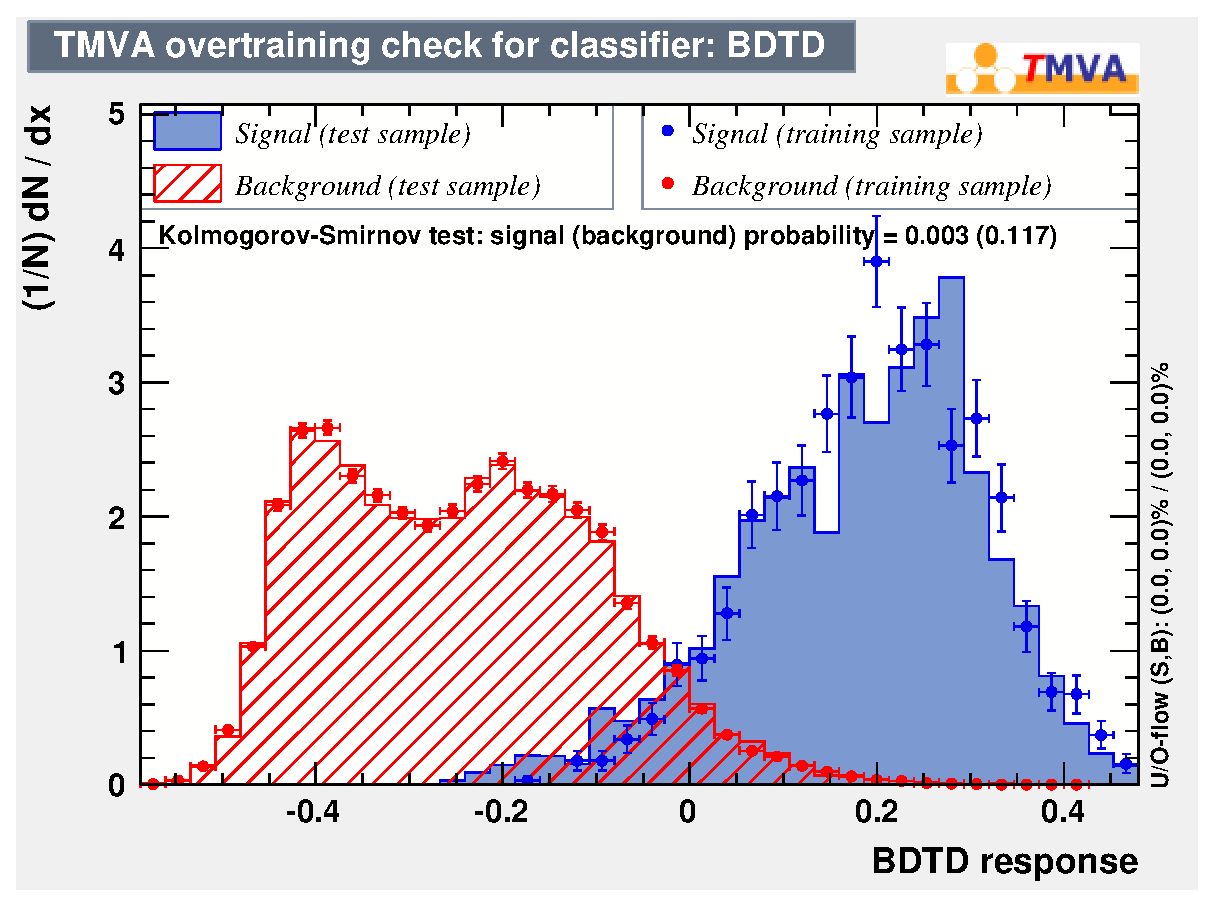
\includegraphics[width=0.5\textwidth]{cutOpt/nonISR_newSample_BDT_dist.eps}
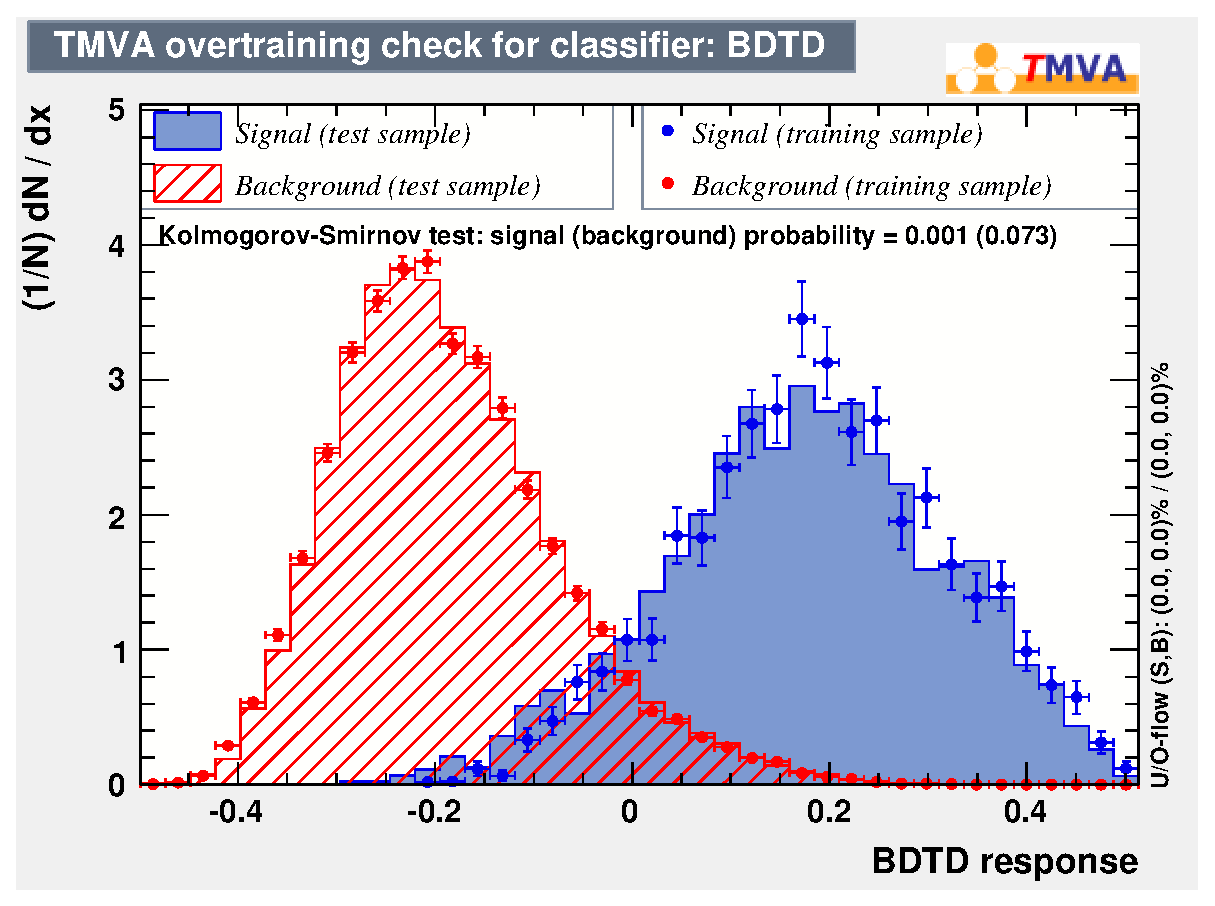
\includegraphics[width=0.5\textwidth]{cutOpt/ISR_newSample_BDT_dist.eps}
\caption{BDT output for nonISR(left) and ISR region(right)}
\label{fig:BDT_output}
\end{figure}

\subsection{Cut optimization}
A cut on BDT output was apllied to define the signal region. Various cut values were tried to find the optimal point. Optimal was defined as having the smallest CLs. To obtain the CLs HistFitter was used. The event counts were projected to 33fb-1 and the expected CLs at that luminosity was calculated. The signal region was blinded during the calculation.

The CLs at various BDT cat value for ISR region is shown in \ref{fig:ISR_BDTCut_CLs}.

\begin{figure}
	\centering
    \begin{subfigure}[b]{0.4\textwidth}
        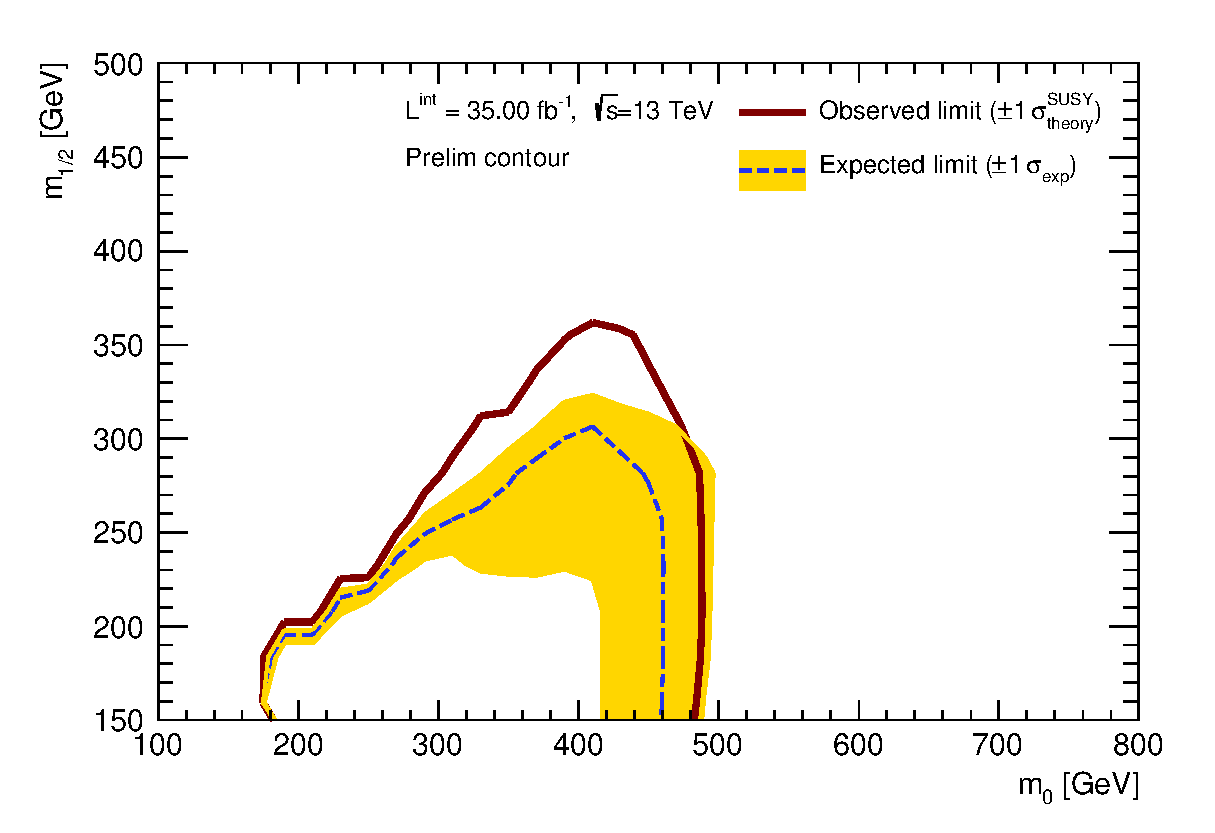
\includegraphics[width=\textwidth]{cutOpt/atlascls_m0m1_wband1_wfixSigXSecband1_showcms0_My2LSSAnalysis_ISR_Alldm_Cut0d1_Output_hypotest__1_harvest_list.eps}
        \caption{}
    \end{subfigure}
    \begin{subfigure}[b]{0.4\textwidth}
        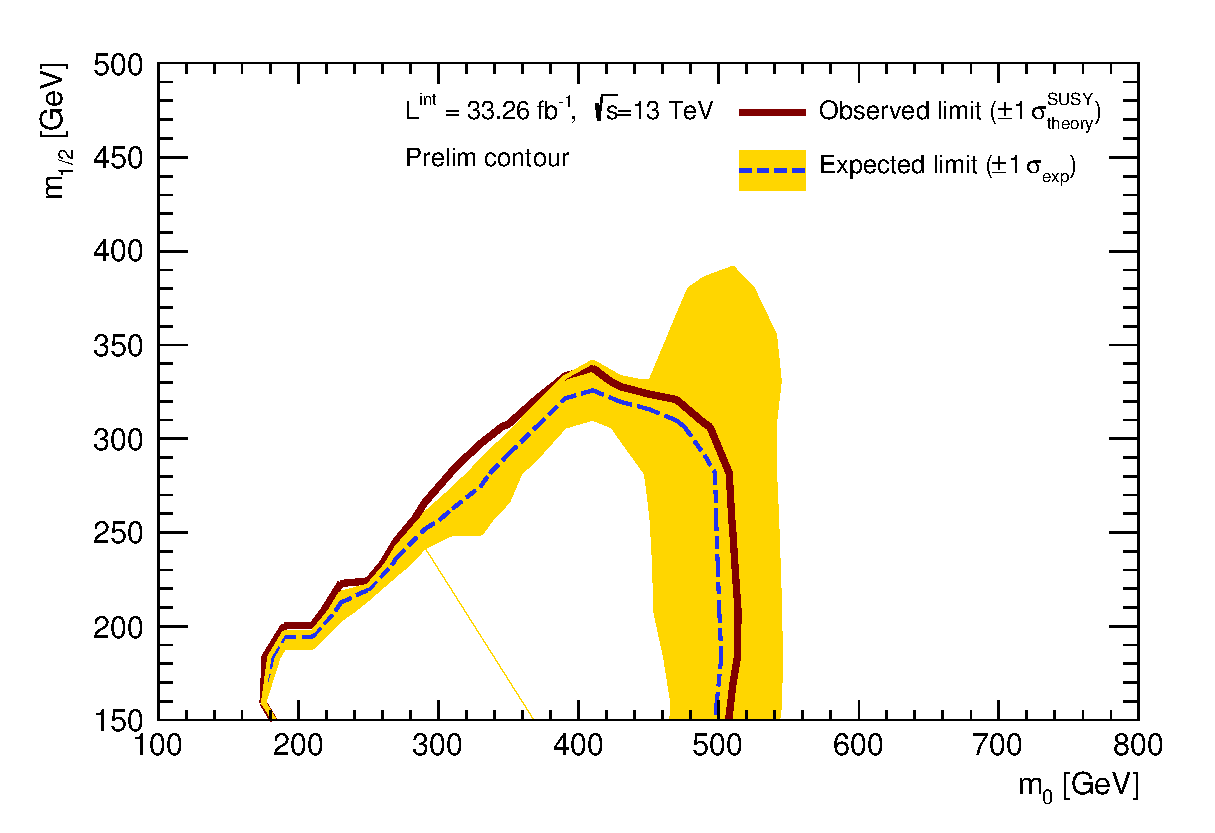
\includegraphics[width=\textwidth]{cutOpt/atlascls_m0m1_wband1_wfixSigXSecband1_showcms0_My2LSSAnalysis_ISR_Alldm_Cut0d2_Output_hypotest__1_harvest_list.eps}
        \caption{}
    \end{subfigure}

    \begin{subfigure}[b]{0.4\textwidth}
        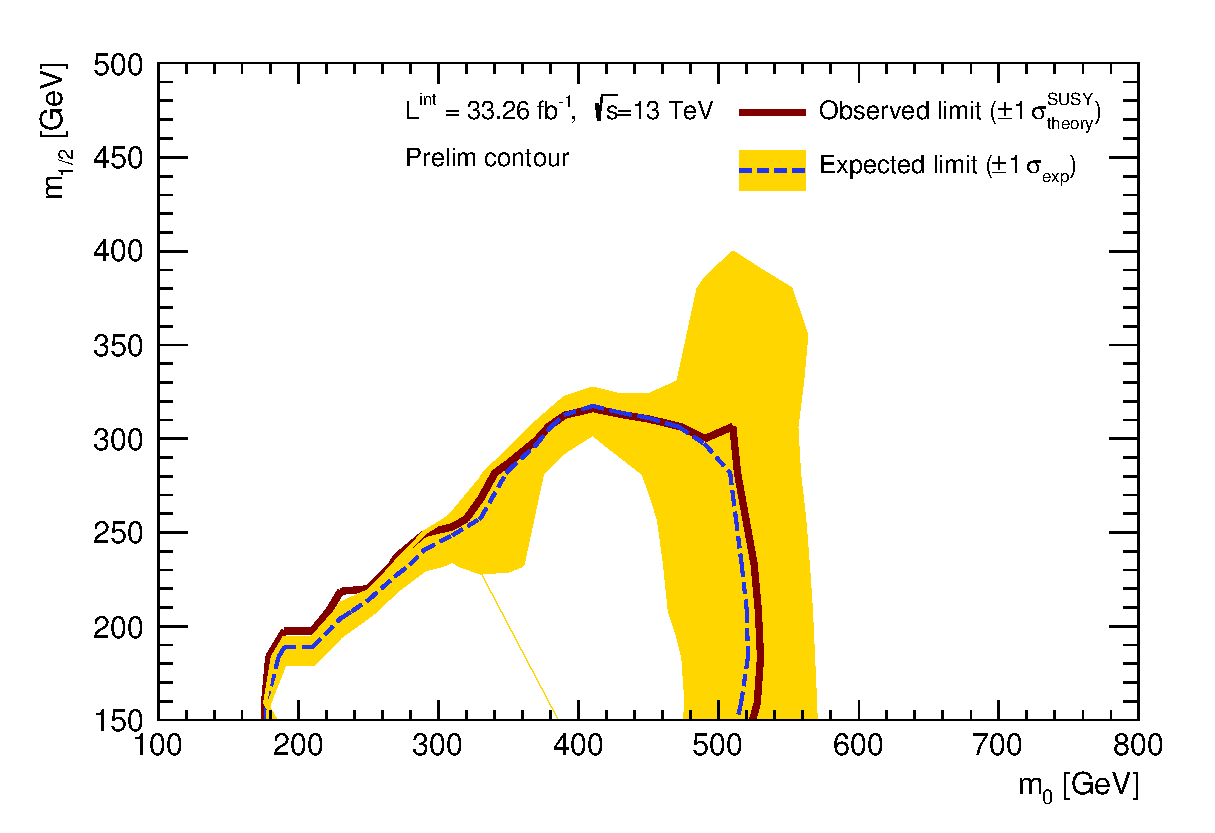
\includegraphics[width=\textwidth]{cutOpt/atlascls_m0m1_wband1_wfixSigXSecband1_showcms0_My2LSSAnalysis_ISR_Alldm_Cut0d3_Output_hypotest__1_harvest_list.eps}
        \caption{}
    \end{subfigure}
    \begin{subfigure}[b]{0.4\textwidth}
        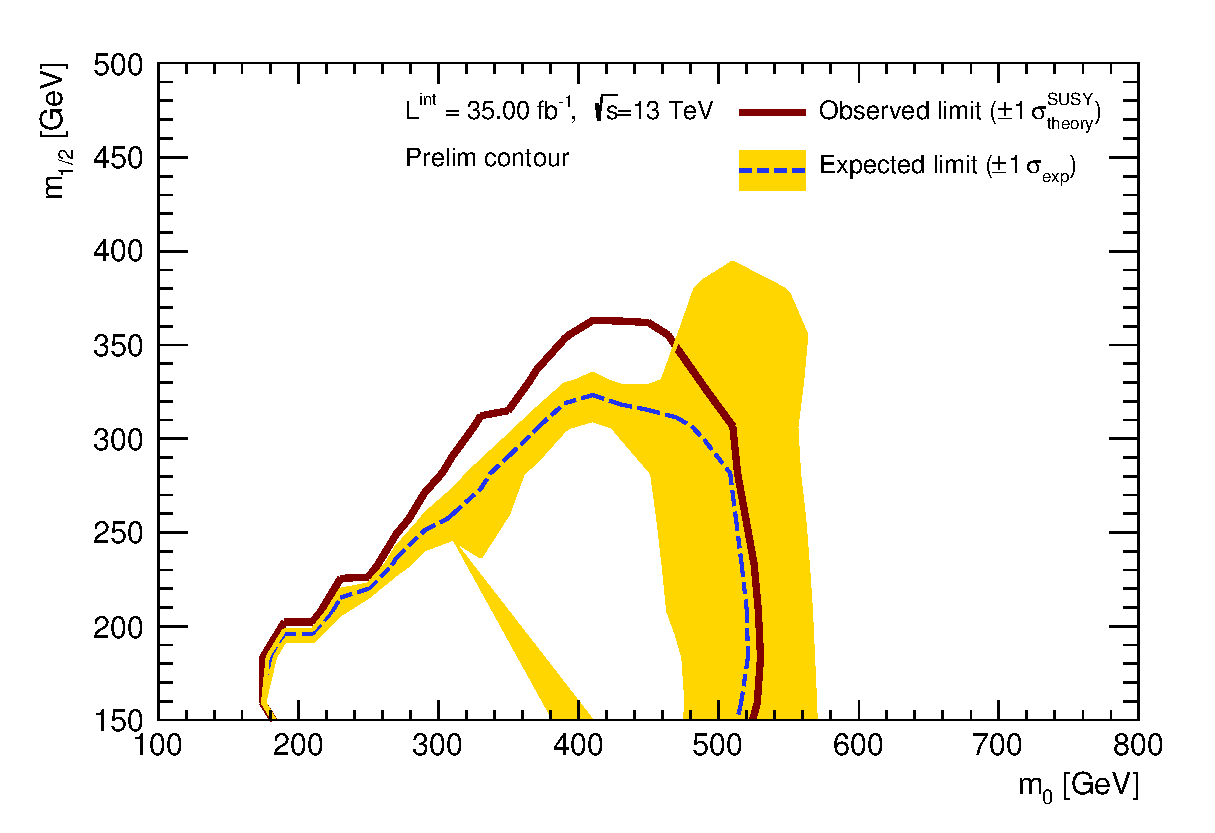
\includegraphics[width=\textwidth]{cutOpt/atlascls_m0m1_wband1_wfixSigXSecband1_showcms0_My2LSSAnalysis_ISR_Alldm_CutOptimal_Output_hypotest__1_harvest_list.eps}
        \caption{}
    \end{subfigure}

\caption{expected CLs for BDT cut at a)0.1 b)0.2 c)0.3 for ISR region. d) combines the three by choosing the best BDT cut at each grid point }
\label{fig:ISR_BDTCut_CLs}
\end{figure}

\begin{figure}
	\centering
    \begin{subfigure}[b]{0.4\textwidth}
        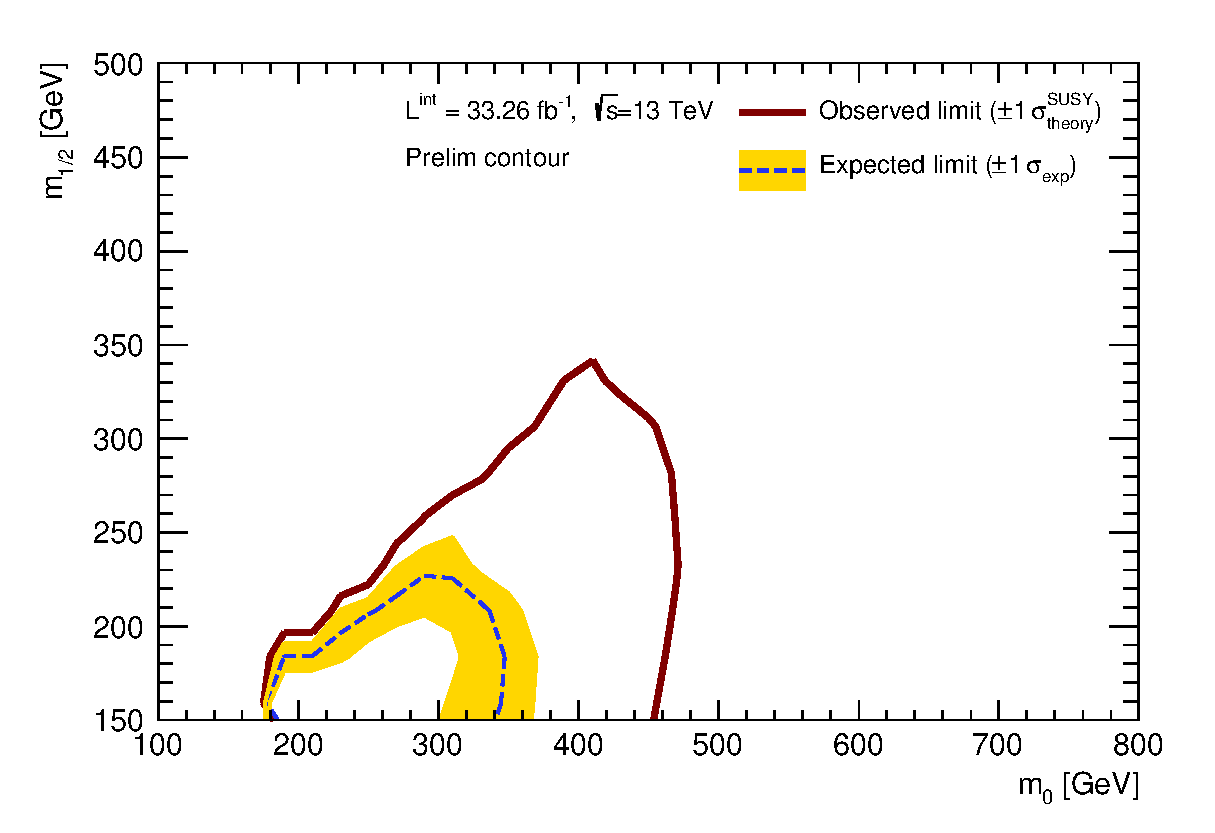
\includegraphics[width=\textwidth]{cutOpt/atlascls_m0m1_wband1_wfixSigXSecband1_showcms0_My2LSSAnalysis_nonISR_Alldm_Cut0d1_Output_hypotest__1_harvest_list.eps}
        \caption{}
    \end{subfigure}
    \begin{subfigure}[b]{0.4\textwidth}
        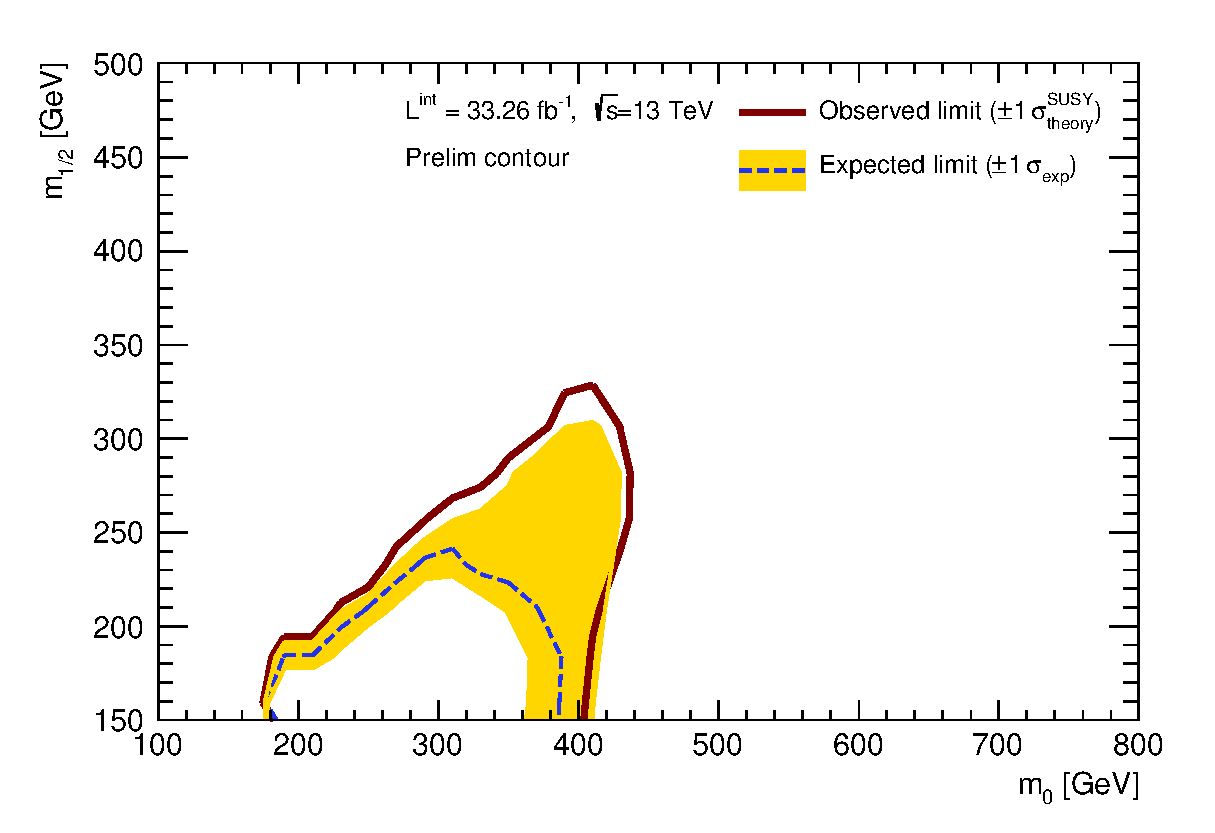
\includegraphics[width=\textwidth]{cutOpt/atlascls_m0m1_wband1_wfixSigXSecband1_showcms0_My2LSSAnalysis_nonISR_Alldm_Cut0d2_Output_hypotest__1_harvest_list.eps}
        \caption{}
    \end{subfigure}

    \begin{subfigure}[b]{0.4\textwidth}
        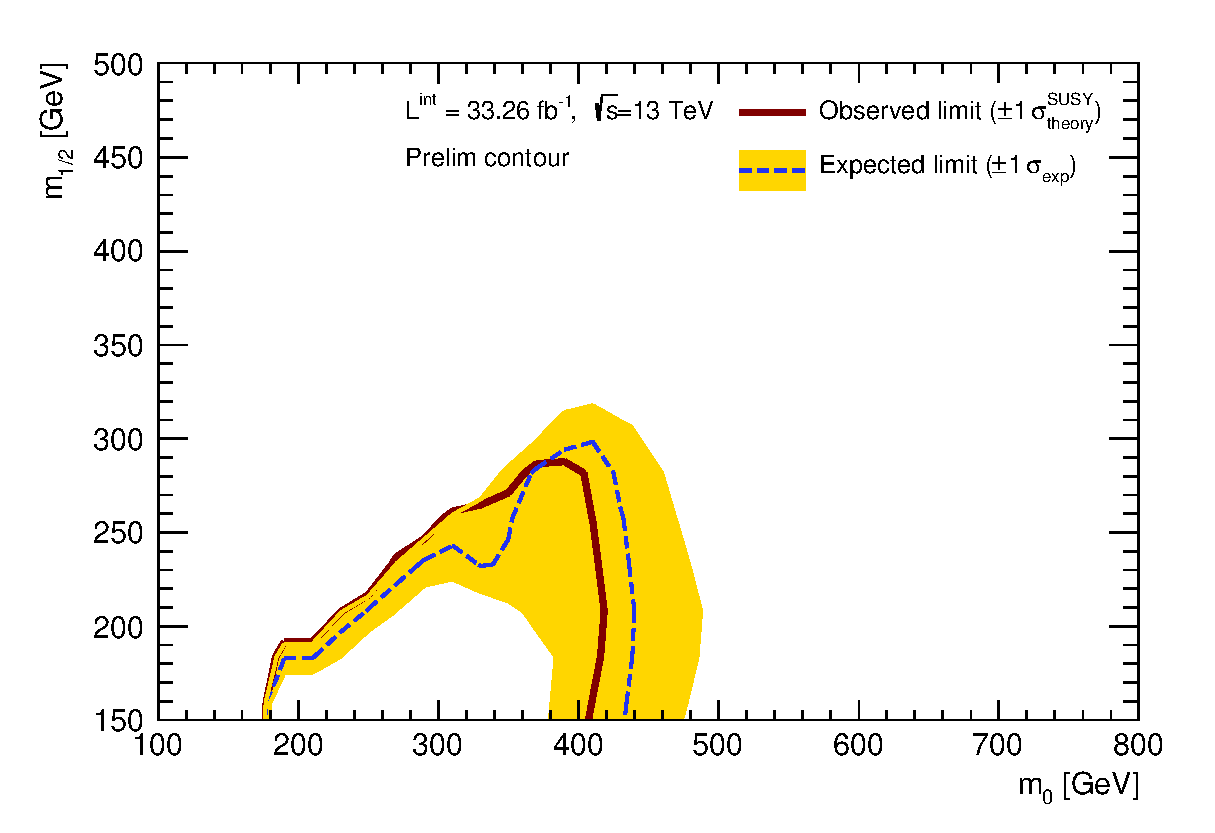
\includegraphics[width=\textwidth]{cutOpt/atlascls_m0m1_wband1_wfixSigXSecband1_showcms0_My2LSSAnalysis_nonISR_Alldm_Cut0d3_Output_hypotest__1_harvest_list.eps}
        \caption{}
    \end{subfigure}
    \begin{subfigure}[b]{0.4\textwidth}
        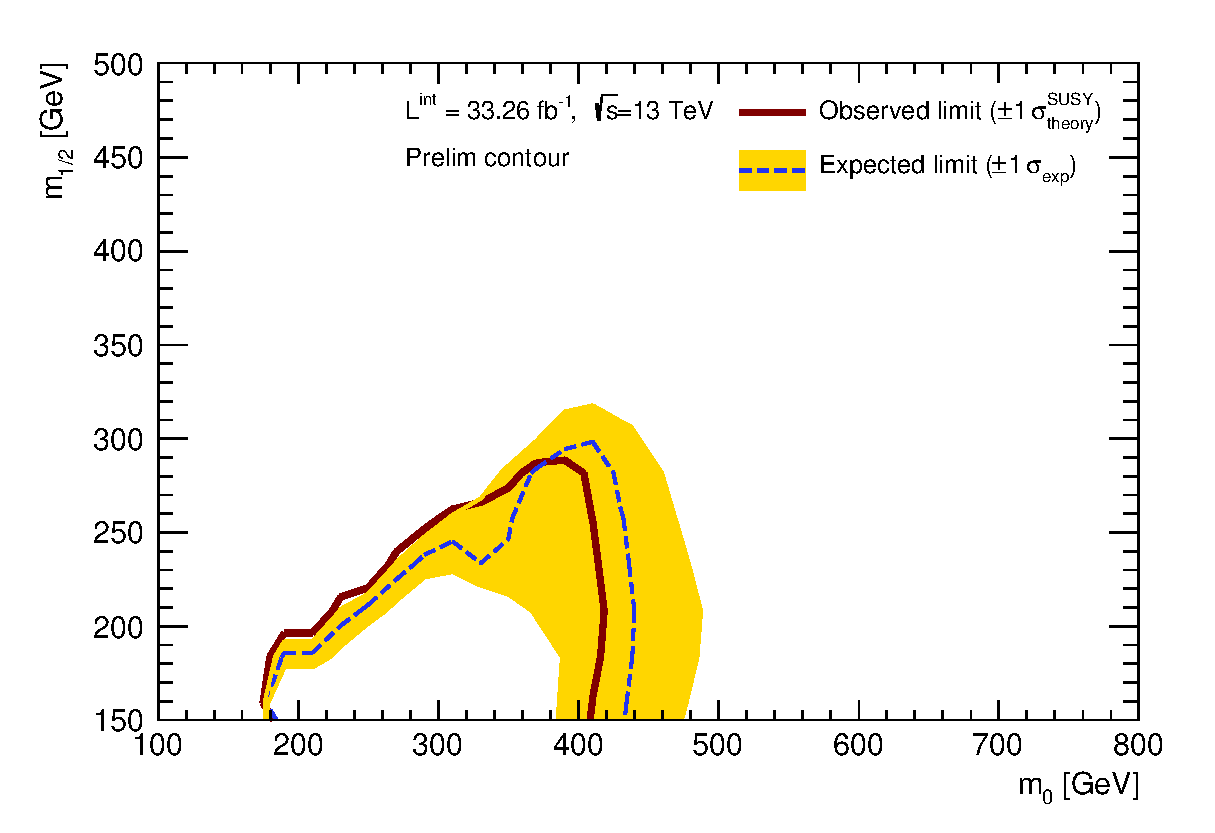
\includegraphics[width=\textwidth]{cutOpt/atlascls_m0m1_wband1_wfixSigXSecband1_showcms0_My2LSSAnalysis_nonISR_Alldm_CutOptimal_Output_hypotest__1_harvest_list.eps}
        \caption{}
    \end{subfigure}

\caption{expected CLs for BDT cut at a)0.1 b)0.2 c)0.3 for nonISR region. d) combines the three by choosing the best BDT cut at each grid point }
\label{fig:nonISR_BDTCut_CLs}
\end{figure}

\subsection{Results}
When both regions are combined, the exclusion plot in \ref{fig:comb_CLs} was obtained.

%FIXME this table is for a particular signal sample only, replace or remove?
\begin{figure}
\centering
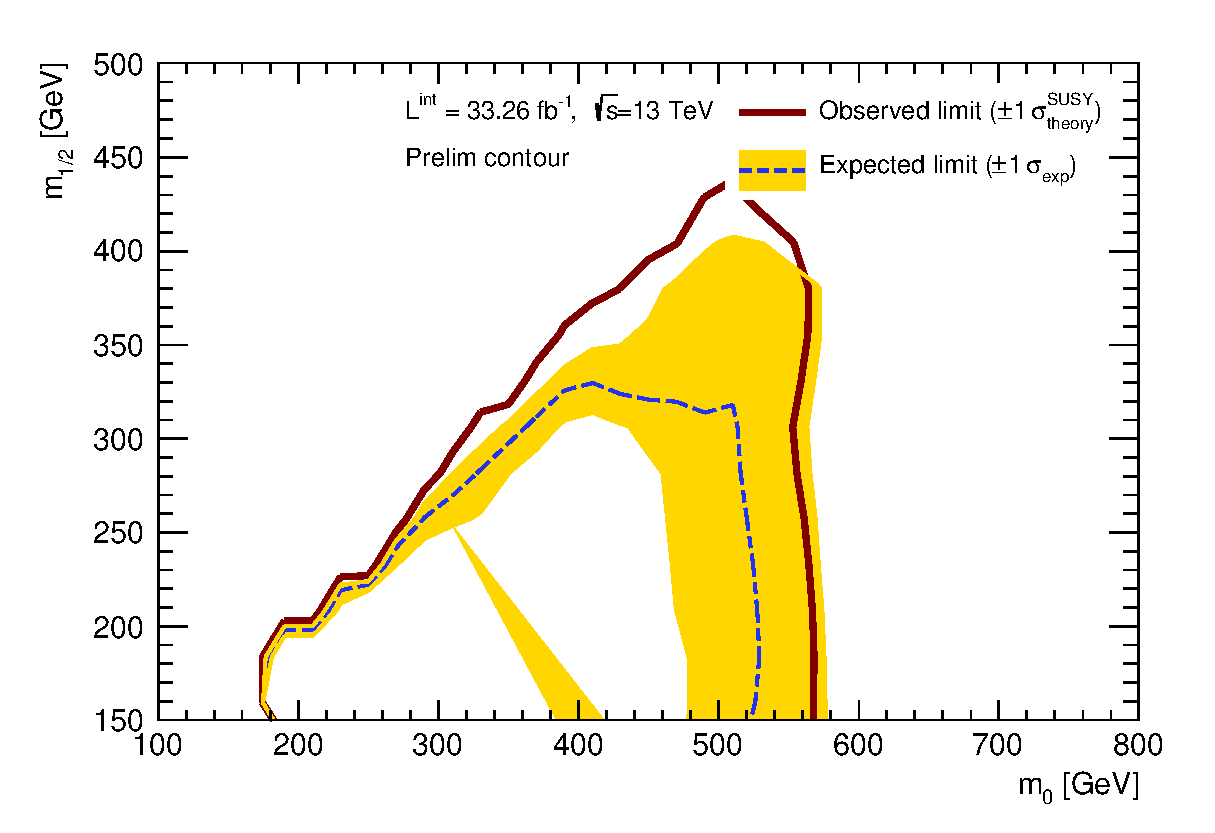
\includegraphics[width=0.8\textwidth]{cutOpt/atlascls_m0m1_wband1_wfixSigXSecband1_showcms0_My2LSSAnalysis_Comb_Alldm_CutOptimal_Output_hypotest__1_harvest_list.eps}
\caption{expected CLs after combining nonISR and ISR region}
\label{fig:comb_CLs}
\end{figure}

\begin{table}
\begin{center}
\setlength{\tabcolsep}{0.0pc}
{\small
%%
\begin{tabular*}{\textwidth}{@{\extracolsep{\fill}}lrr}
\noalign{\smallskip}\hline\noalign{\smallskip}
{\bf table.results.yields channel}           & SRISR            & SRnonISR              \\[-0.05cm]
\noalign{\smallskip}\hline\noalign{\smallskip}
%%
Observed events          & $1$              & $7$                    \\
\noalign{\smallskip}\hline\noalign{\smallskip}
%%
Fitted bkg events         & $1.56_{-1.56}^{+1.96}$          & $7.20 \pm 2.57$              \\
\noalign{\smallskip}\hline\noalign{\smallskip}
%%
        Fitted BDT\_MGPy8EG\_A14N23LO\_C1N2\_Slep\_400\_300\_Data\_ events         & $0.05_{-0.05}^{+1.99}$          & $0.06_{-0.06}^{+2.51
}$              \\
%%
        Fitted BDT\_CFlip\_ events         & $0.18 \pm 0.03$          & $0.56 \pm 0.08$              \\
%%
        Fitted BDT\_fakeLep\_ events         & $0.00 \pm 0.00$          & $0.00 \pm 0.00$              \\
%%
        Fitted BDT\_diboson\_Data\_ events         & $1.19 \pm 0.25$          & $3.64 \pm 0.62$              \\
%%
        Fitted BDT\_wgamma\_Data events         & $0.12_{-0.12}^{+0.19}$          & $0.95 \pm 0.25$              \\
%%
        Fitted BDT\_ttbar\_Data\_ events         & $0.03 \pm 0.01$          & $0.01 \pm 0.00$              \\
%%
 \noalign{\smallskip}\hline\noalign{\smallskip}
%%
MC exp. SM events              & $6.93$          & $13.99$              \\
\noalign{\smallskip}\hline\noalign{\smallskip}
%%
        MC exp. BDT\_MGPy8EG\_A14N23LO\_C1N2\_Slep\_400\_300\_Data\_ events         & $5.42$          & $6.86$              \\
%%
        MC exp. BDT\_CFlip\_ events         & $0.18$          & $0.56$              \\
%%
        MC exp. BDT\_fakeLep\_ events         & $0.00$          & $0.00$              \\
%%
        MC exp. BDT\_diboson\_Data\_ events         & $1.19$          & $3.63$              \\
%%
        MC exp. BDT\_wgamma\_Data events         & $0.12$          & $0.95$              \\
%%
        MC exp. BDT\_ttbar\_Data\_ events         & $0.03$          & $0.01$              \\
%%     \\
\noalign{\smallskip}\hline\noalign{\smallskip}
\end{tabular*}
%%%
}
\end{center}

\caption{Signal region: . Fit results for an integrated luminosity of $1035$\,\ipb.
}
\label{table.results.systematics.in.logL.fit.table.results.yields}
\end{table}
%



\begin{table}
\begin{center}
\setlength{\tabcolsep}{0.0pc}
\begin{tabular*}{\textwidth}{@{\extracolsep{\fill}}lcc}
\noalign{\smallskip}\hline\noalign{\smallskip}
{\bf Uncertainty of channel}                                    & SRISR            & SRnonISR            \\
\noalign{\smallskip}\hline\noalign{\smallskip}
%%
Total background expectation             &  $1.56$        &  $7.20$       \\
%% \\
\noalign{\smallskip}\hline\noalign{\smallskip}
%%
Total statistical $(\sqrt{N_{\rm exp}})$              & $\pm 1.25$        & $\pm 2.68$       \\
%%
Total background systematic               & $\pm 1.96\ [125.57\%] $        & $\pm 2.57\ [35.64\%] $             \\
\noalign{\smallskip}\hline\noalign{\smallskip}
\noalign{\smallskip}\hline\noalign{\smallskip}
%%
mu\_SIG         & $\pm 1.99$          & $\pm 2.51$       \\
%%
gamma\_stat\_SRISR\_cuts\_bin\_0         & $\pm 0.22$          & $\pm 0.00$       \\
%%
alpha\_JET\_GroupedNP\_1         & $\pm 0.10$          & $\pm 0.27$       \\
%%
alpha\_EG\_RESOLUTION         & $\pm 0.08$          & $\pm 0.03$       \\
%%
alpha\_MUONS\_MS         & $\pm 0.06$          & $\pm 0.05$       \\
%%
alpha\_JET\_GroupedNP\_2         & $\pm 0.06$          & $\pm 0.03$       \\
%%
alpha\_MET\_SoftTrk\_Scale         & $\pm 0.06$          & $\pm 0.09$       \\
%%
Lumi         & $\pm 0.05$          & $\pm 0.18$       \\
%%
alpha\_JET\_GroupedNP\_3         & $\pm 0.04$          & $\pm 0.28$       \\
%%
alpha\_EL\_EFF\_ID         & $\pm 0.03$          & $\pm 0.07$       \\
%%
alpha\_MUONS\_ID         & $\pm 0.02$          & $\pm 0.02$       \\
%%
alpha\_EL\_EFF\_Trigger         & $\pm 0.02$          & $\pm 0.05$       \\
%%
alpha\_EL\_EFF\_Iso         & $\pm 0.01$          & $\pm 0.03$       \\
%%
alpha\_MUON\_EFF\_TrigStat         & $\pm 0.01$          & $\pm 0.04$       \\
%%
alpha\_EL\_EFF\_Reco         & $\pm 0.01$          & $\pm 0.03$       \\
%%
alpha\_MUON\_EFF\_TrigSyst         & $\pm 0.01$          & $\pm 0.02$       \\
%%
alpha\_MUON\_EFF\_SYS         & $\pm 0.01$          & $\pm 0.02$       \\
%%
alpha\_EG\_SCALE         & $\pm 0.00$          & $\pm 0.02$       \\
%%
alpha\_CFlip\_0         & $\pm 0.00$          & $\pm 0.00$       \\
%%
alpha\_MUON\_EFF\_STAT         & $\pm 0.00$          & $\pm 0.01$       \\
%%
alpha\_MUON\_ISO\_SYS         & $\pm 0.00$          & $\pm 0.00$       \\
%%
alpha\_MUON\_ISO\_STAT         & $\pm 0.00$          & $\pm 0.00$       \\
%%
alpha\_PRW\_DATASF         & $\pm 0.00$          & $\pm 0.00$       \\
%%
alpha\_MET\_SoftTrk\_ResoPara         & $\pm 0.00$          & $\pm 0.00$       \\
%%
alpha\_MET\_SoftTrk\_ResoPerp         & $\pm 0.00$          & $\pm 0.00$       \\
%%
alpha\_FakeLep\_0         & $\pm 0.00$          & $\pm 0.07$       \\
%%
alpha\_JET\_JER\_SINGLE\_NP         & $\pm 0.00$          & $\pm 0.00$       \\
%%
alpha\_MUONS\_SCALE         & $\pm 0.00$          & $\pm 0.08$       \\
%%
gamma\_stat\_SRnonISR\_cuts\_bin\_0         & $\pm 0.00$          & $\pm 1.02$       \\
%%
\noalign{\smallskip}\hline\noalign{\smallskip}
\end{tabular*}
\end{center}

\caption[Breakdown of uncertainty on background estimates]{
Breakdown of the dominant systematic uncertainties on background estimates in the various signal regions.
Note that the individual uncertainties can be correlated, and do not necessarily add up quadratically to
the total background uncertainty. The percentages show the size of the uncertainty relative to the total expected background.
\label{table.results.bkgestimate.uncertainties.SR}}
\end{table}
%
